% =====================================================================
%  Figure & table FLOATS for the paper (concise captions only; the
%  discussion lives in experiments.tex). Paths are relative to docs/paper/.
% =====================================================================

\begin{figure}[t]\centering
  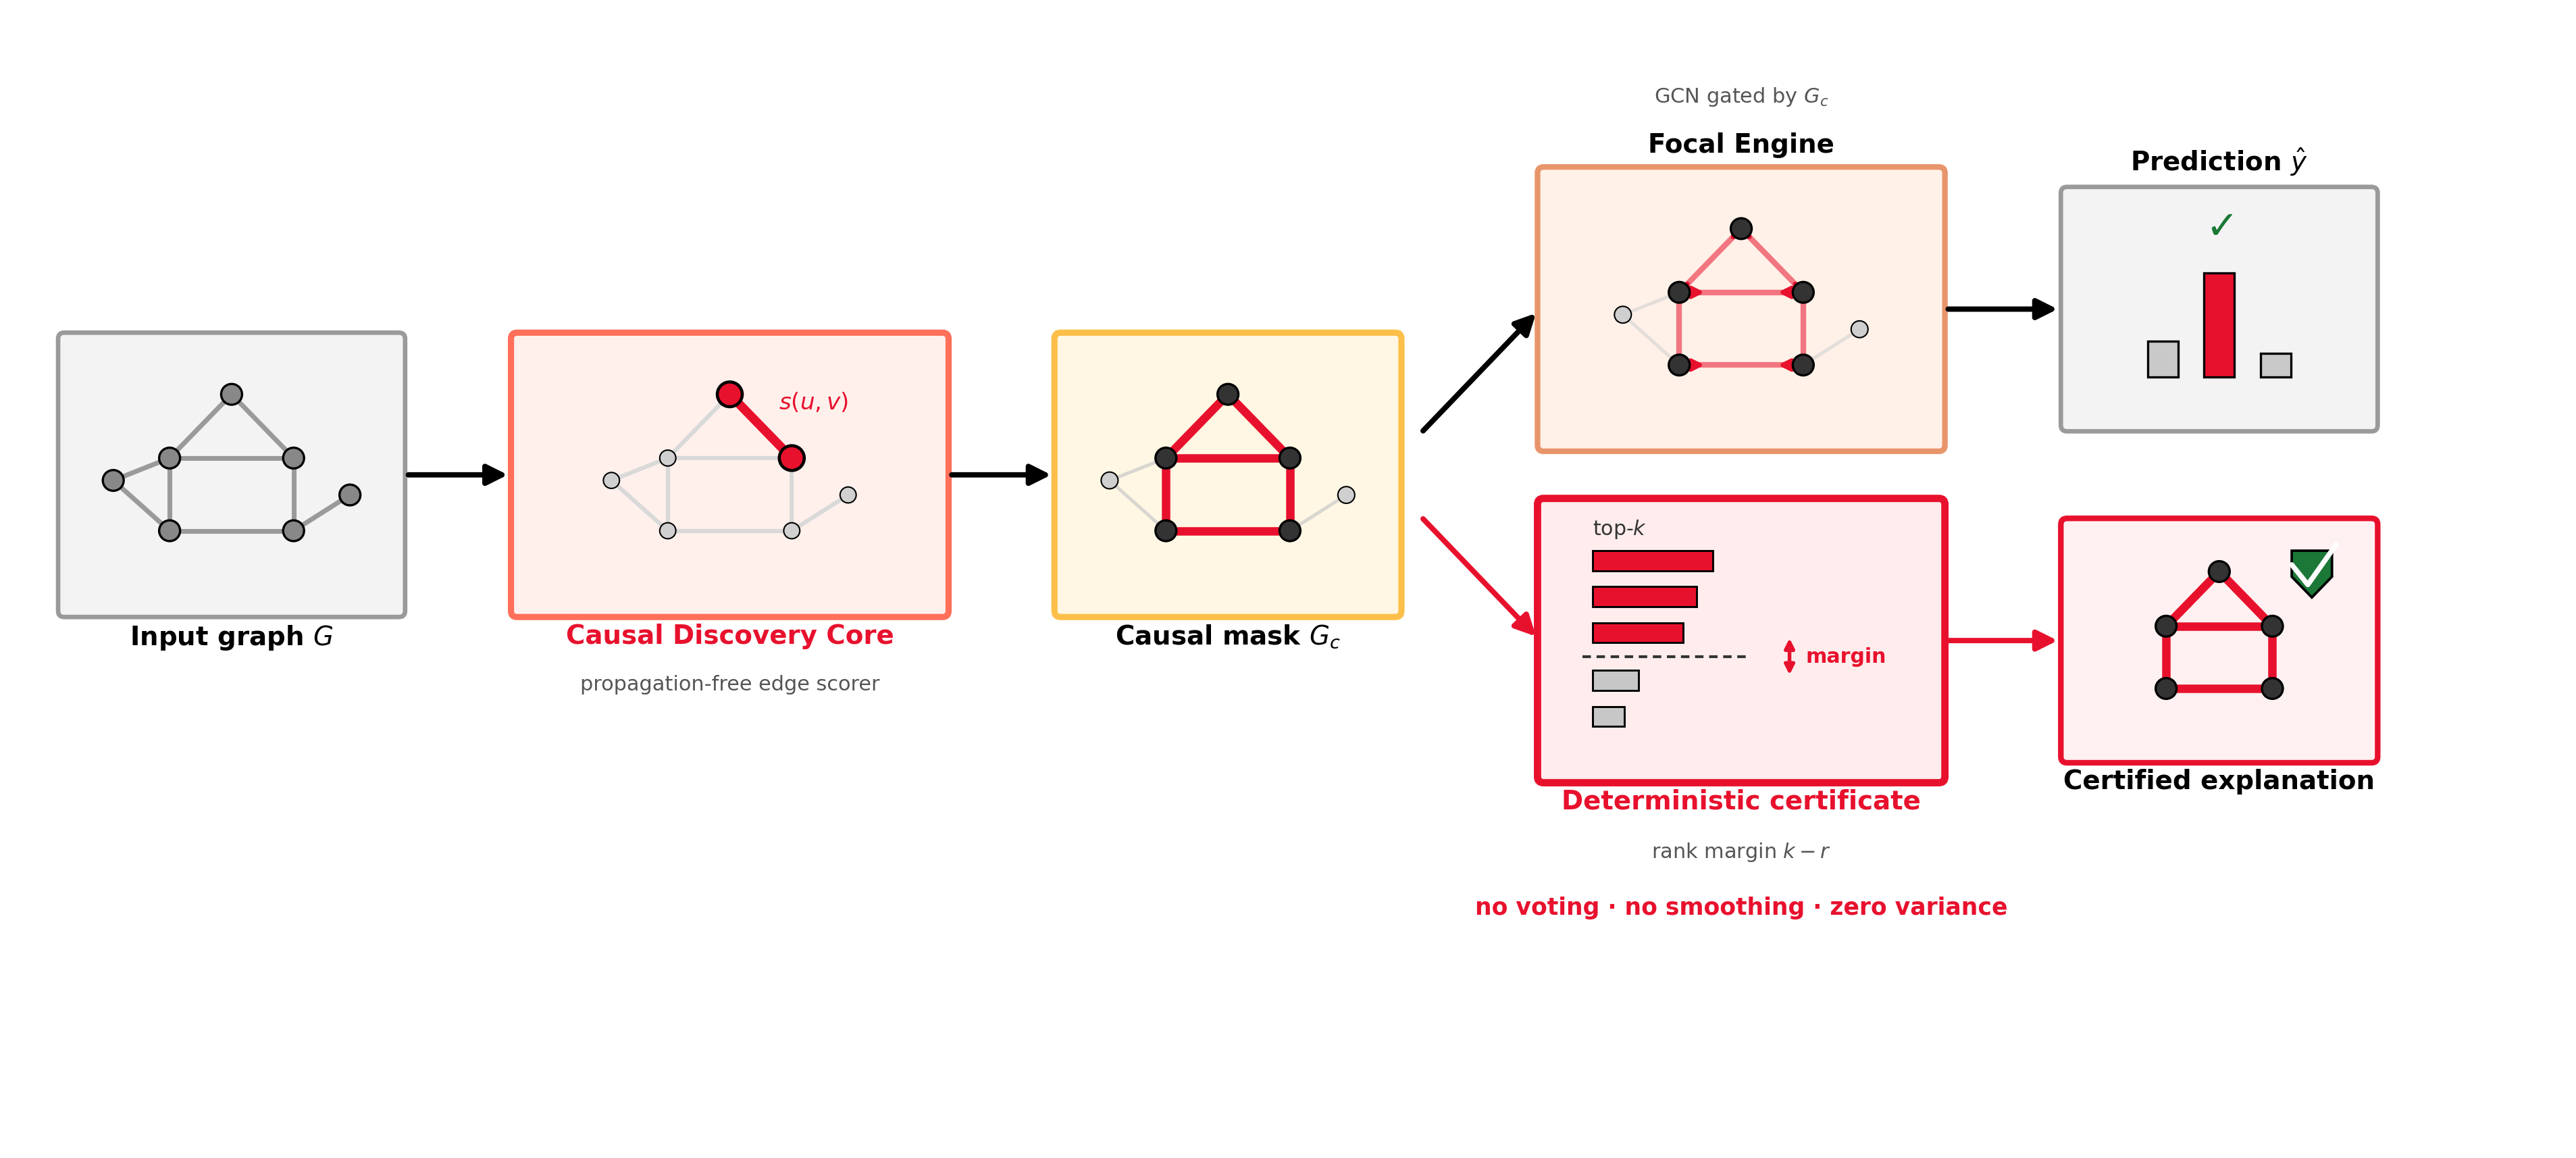
\includegraphics[width=\linewidth]{../../figures/F0_architecture.png}
  \caption{The \aeth{} pipeline: a propagation-free causal core scores each edge
  from its endpoints alone, producing a mask that gates prediction and feeds a
  \emph{deterministic} rank-margin certificate ($k-r$)---no voting, no
  smoothing.}
  \label{fig:arch}
\end{figure}

\begin{figure}[t]\centering
  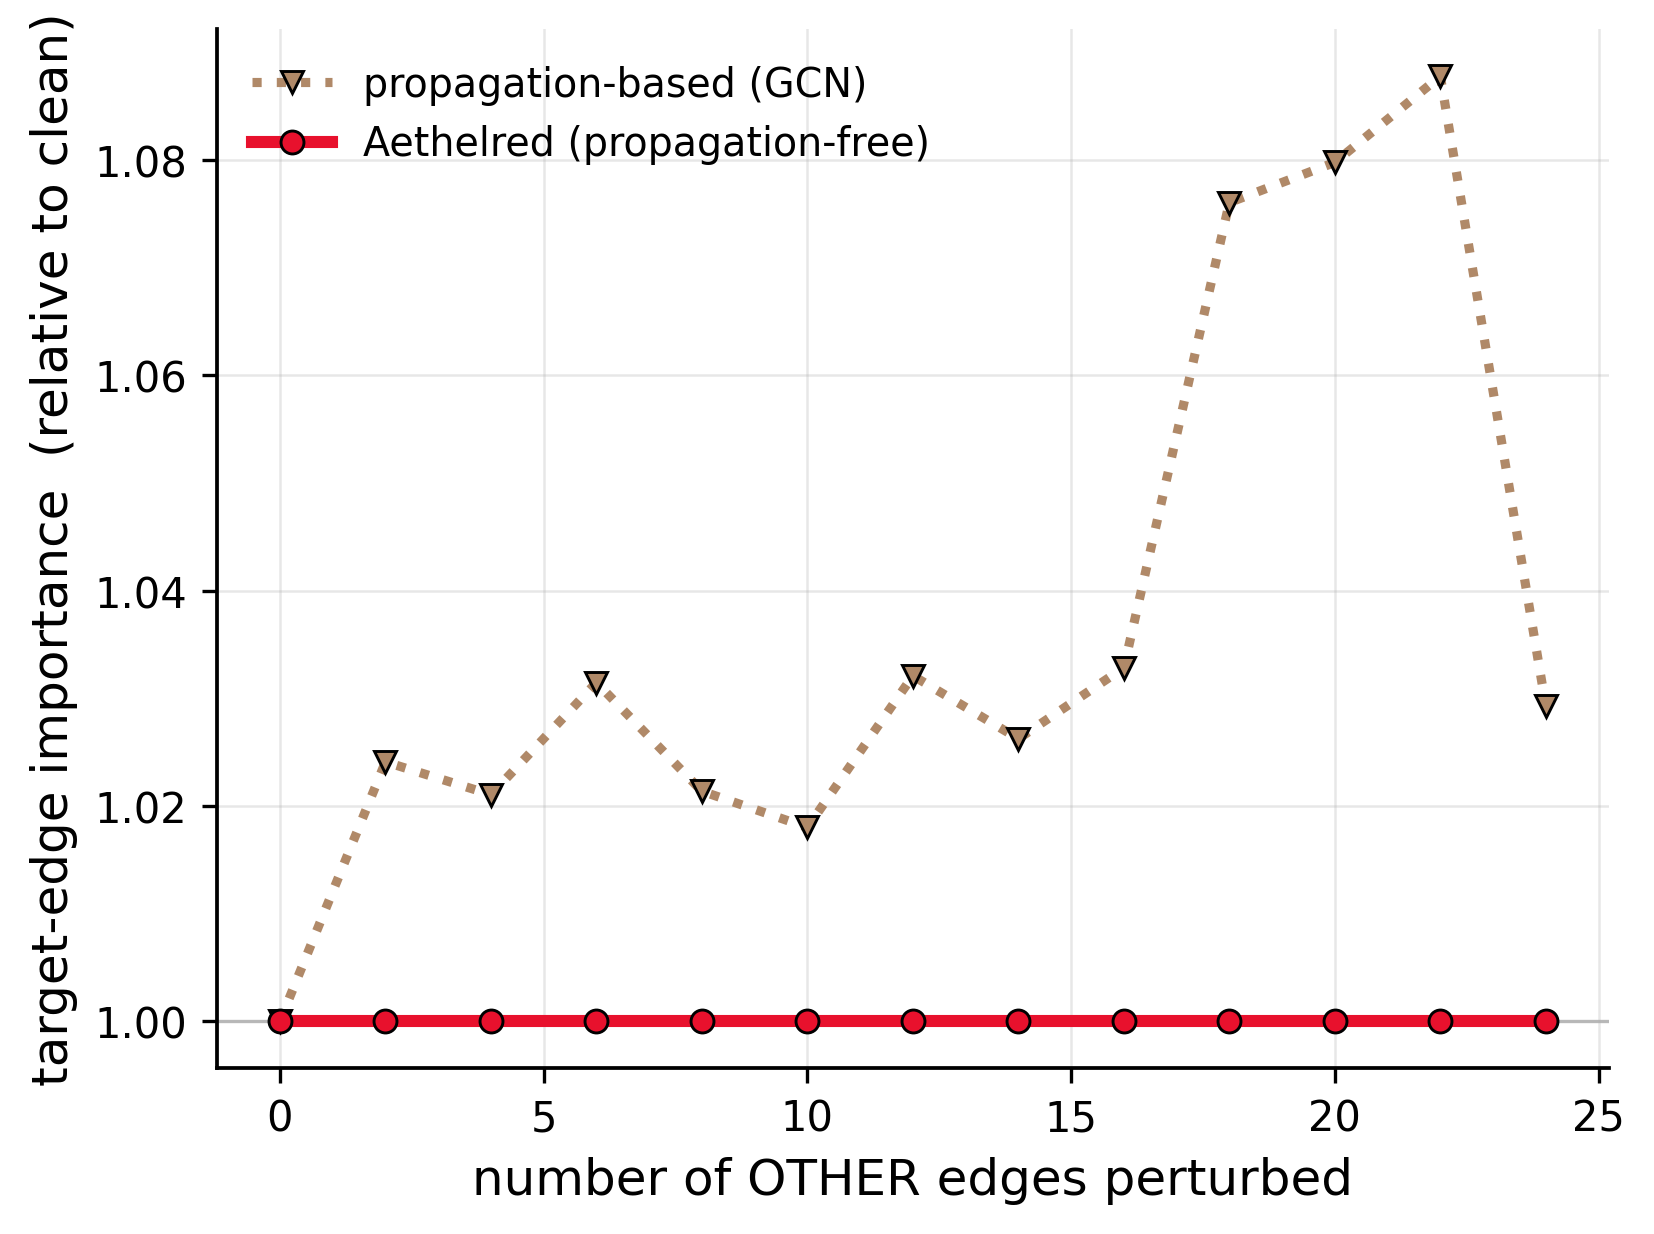
\includegraphics[width=0.82\linewidth]{../../figures/F10_edge_locality.png}
  \caption{Edge-locality. A target edge's importance vs.\ the number of
  \emph{other} edges perturbed: \aeth{}'s score is exactly invariant; a
  propagation-based (GCN) score drifts.}
  \label{fig:locality}
\end{figure}

\begin{figure}[t]\centering
  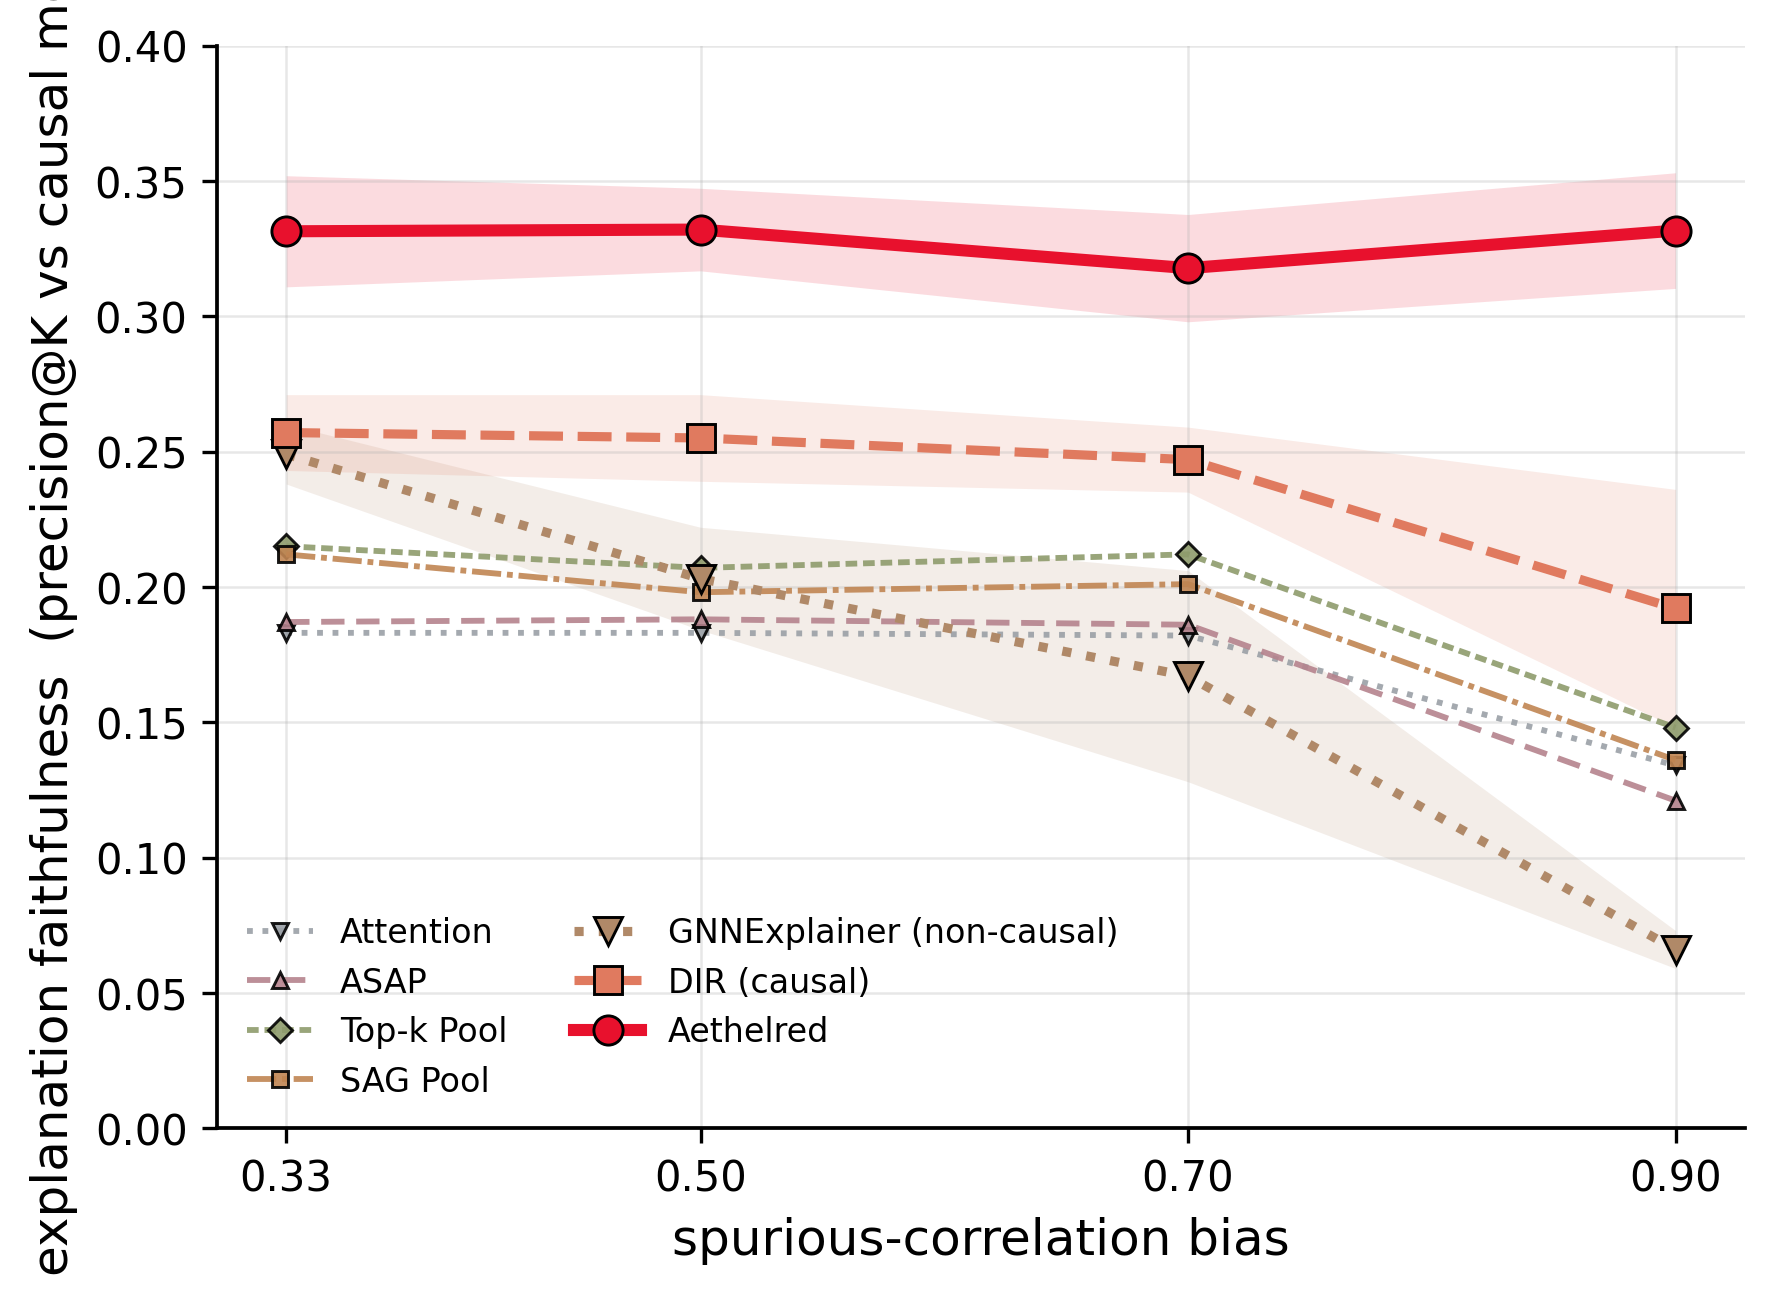
\includegraphics[width=0.9\linewidth]{../../figures/F9_spmotif_causal_vs_spurious.png}
  \caption{Faithfulness (precision@$K$ vs.\ the \emph{causal} motif) as spurious
  correlation strengthens on \textsc{SPMotif}. GNNExplainer and the pooling
  rationale baselines (Attention/ASAP/Top-k/SAG, DIR Table~2) collapse, DIR
  partly resists; \aeth{} is bias-invariant.}
  \label{fig:thesis}
\end{figure}

\begin{figure}[t]\centering
  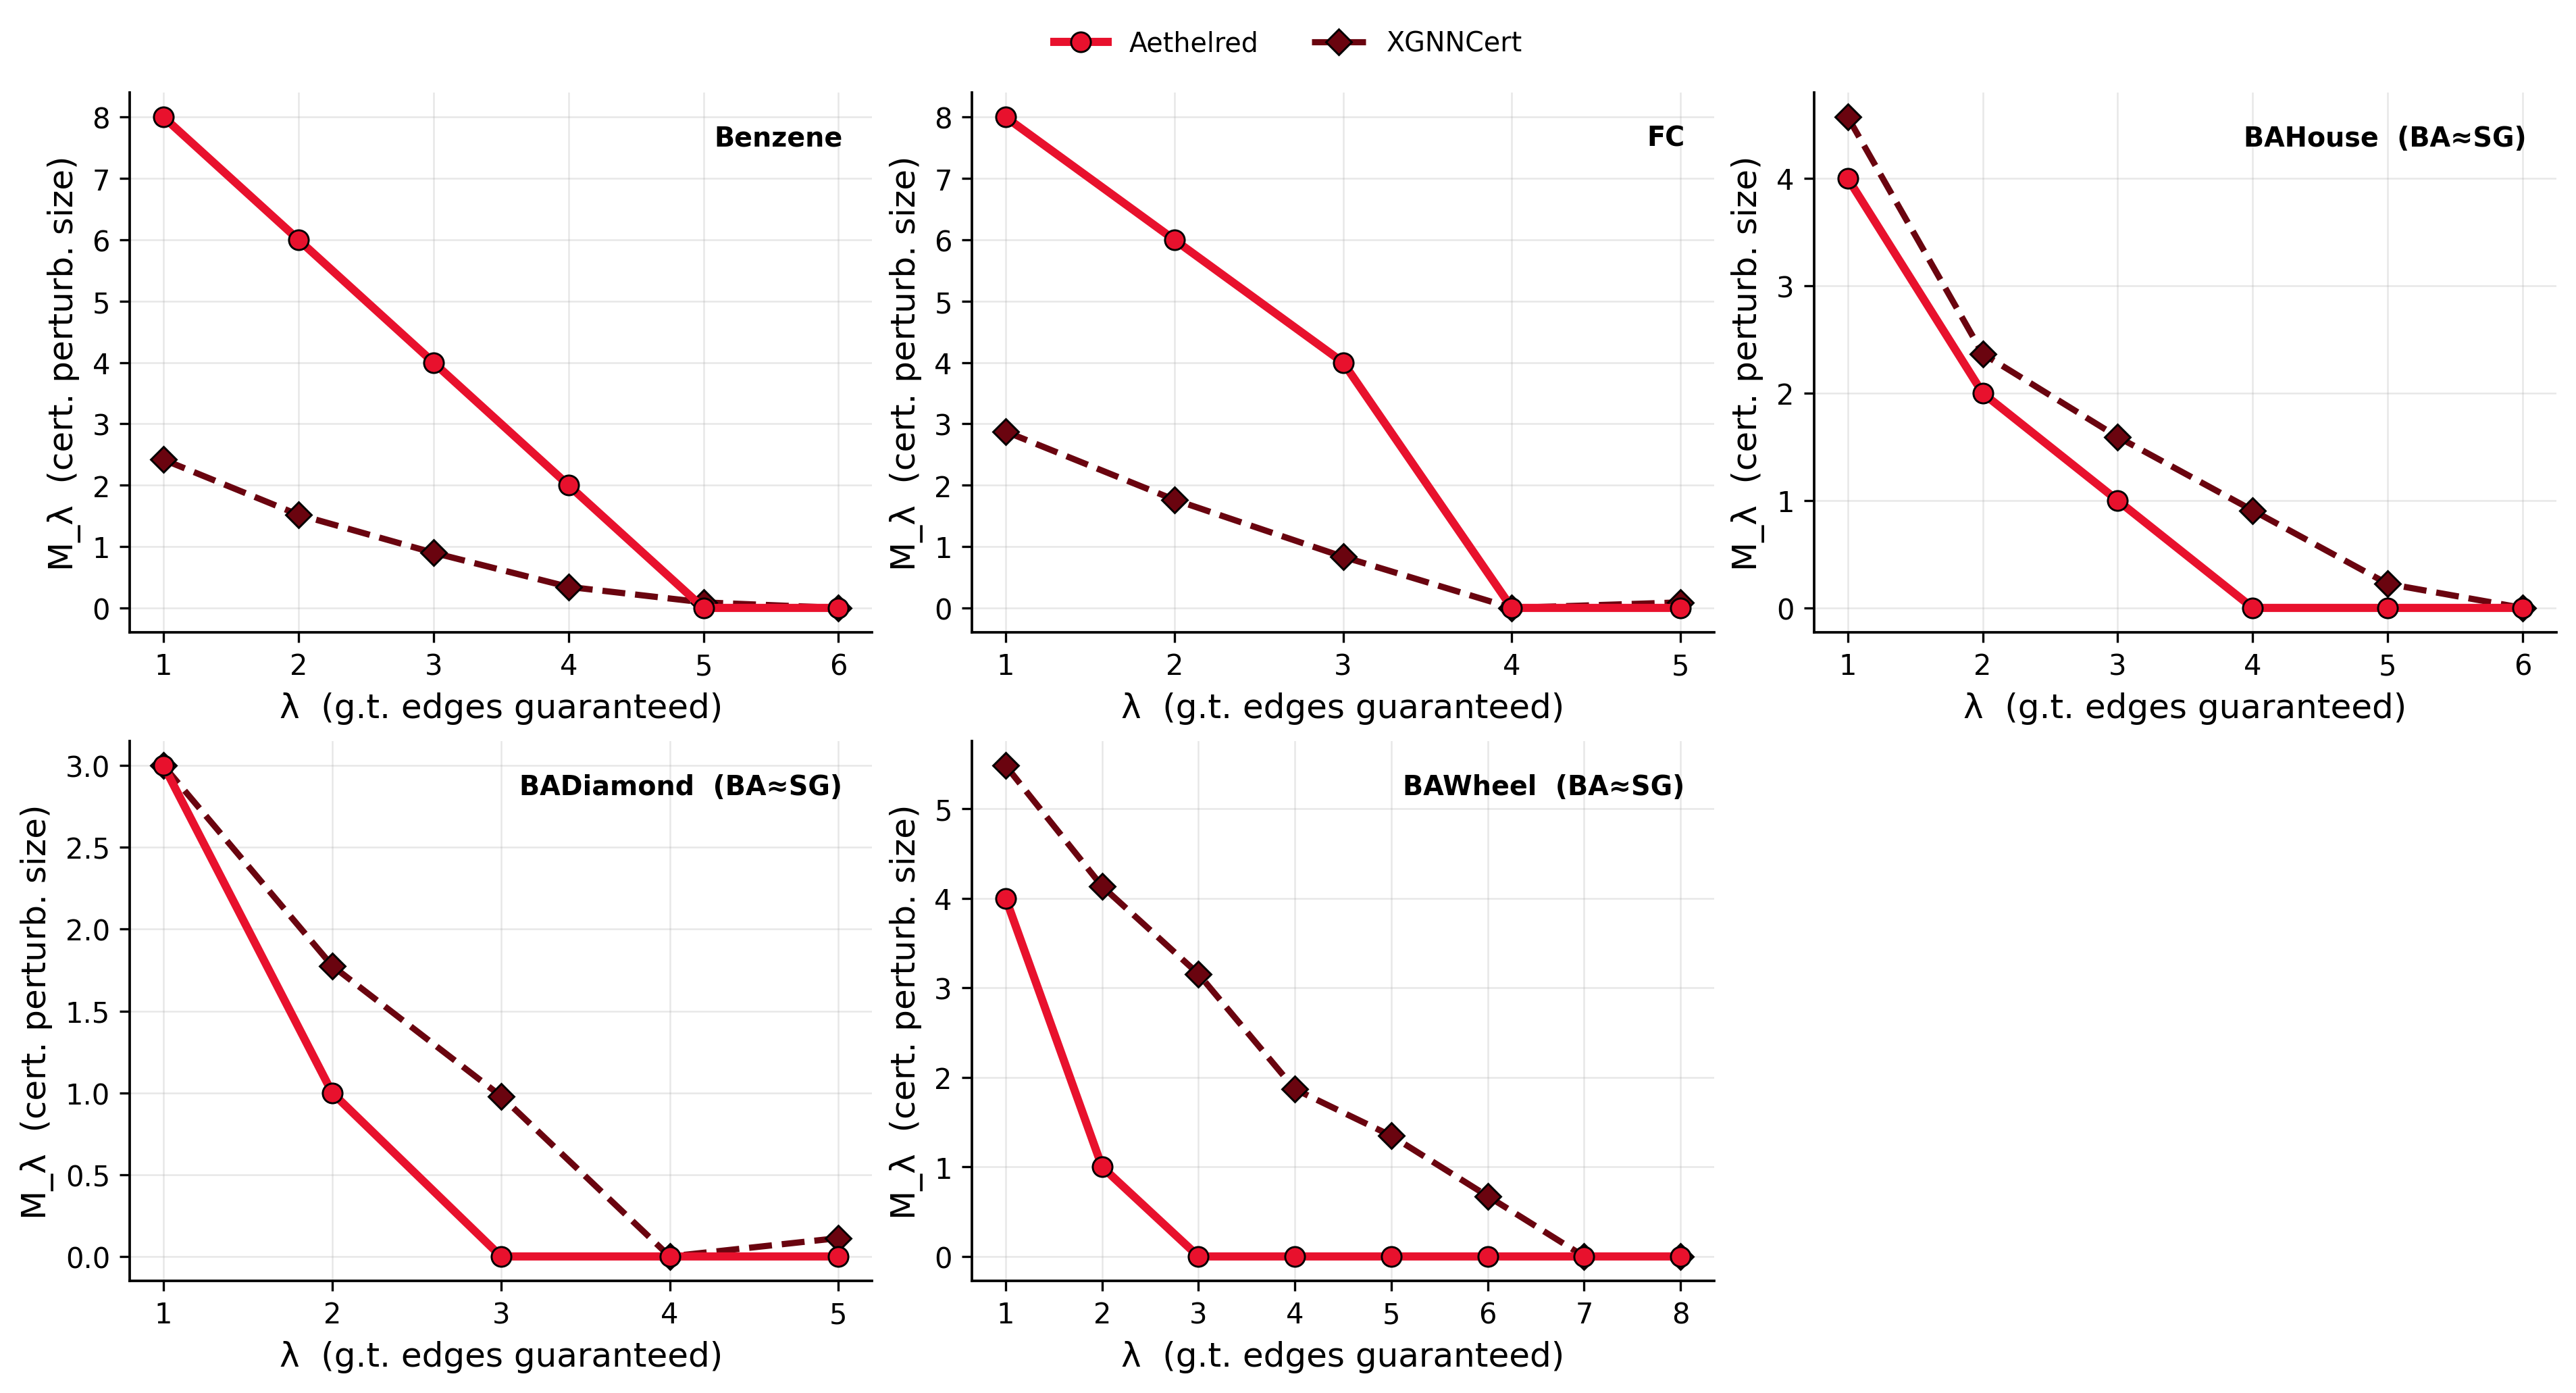
\includegraphics[width=\linewidth]{../../figures/F7_Mlambda_vs_lambda.png}
  \caption{Certified perturbation size $M_\lambda$ vs.\ guaranteed ground-truth
  edges $\lambda$ (\xgn{}'s own metric). \aeth{} vs.\ \xgn{}'s authoritative
  published default ($T{=}70$, PGExplainer).}
  \label{fig:mlambda}
\end{figure}

\begin{figure}[t]\centering
  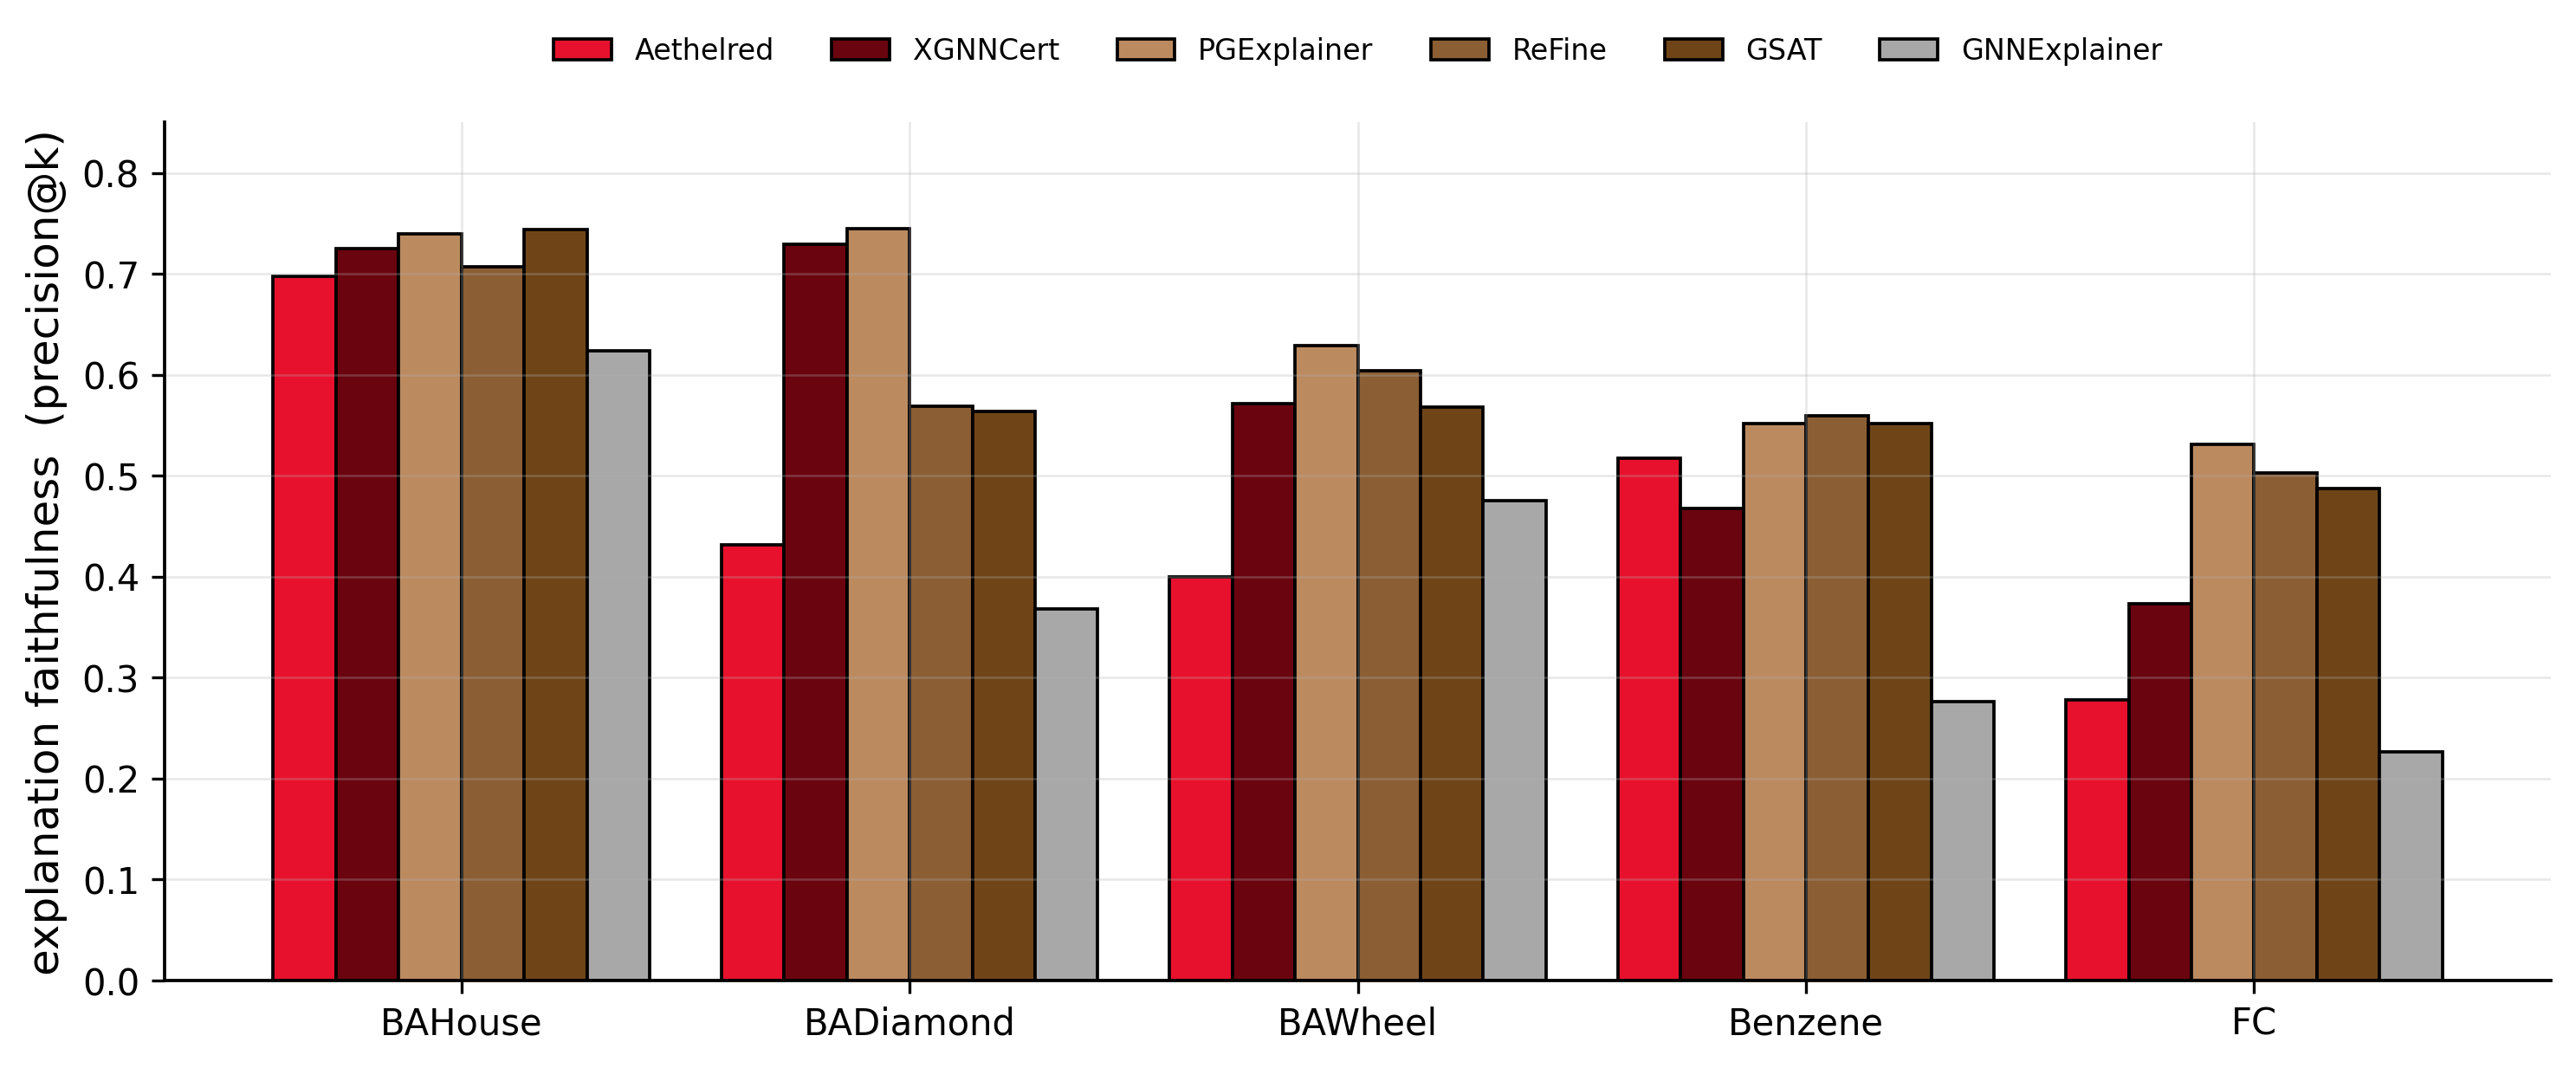
\includegraphics[width=\linewidth]{../../figures/F2c_unified_faithfulness.png}
  \caption{Clean explanation faithfulness: \aeth{} against all explanation
  baselines (\xgn{}, PGExplainer, ReFine, GSAT, GNNExplainer) on the five
  ground-truth-motif datasets.}
  \label{fig:unifaith}
\end{figure}

\begin{figure}[t]\centering
  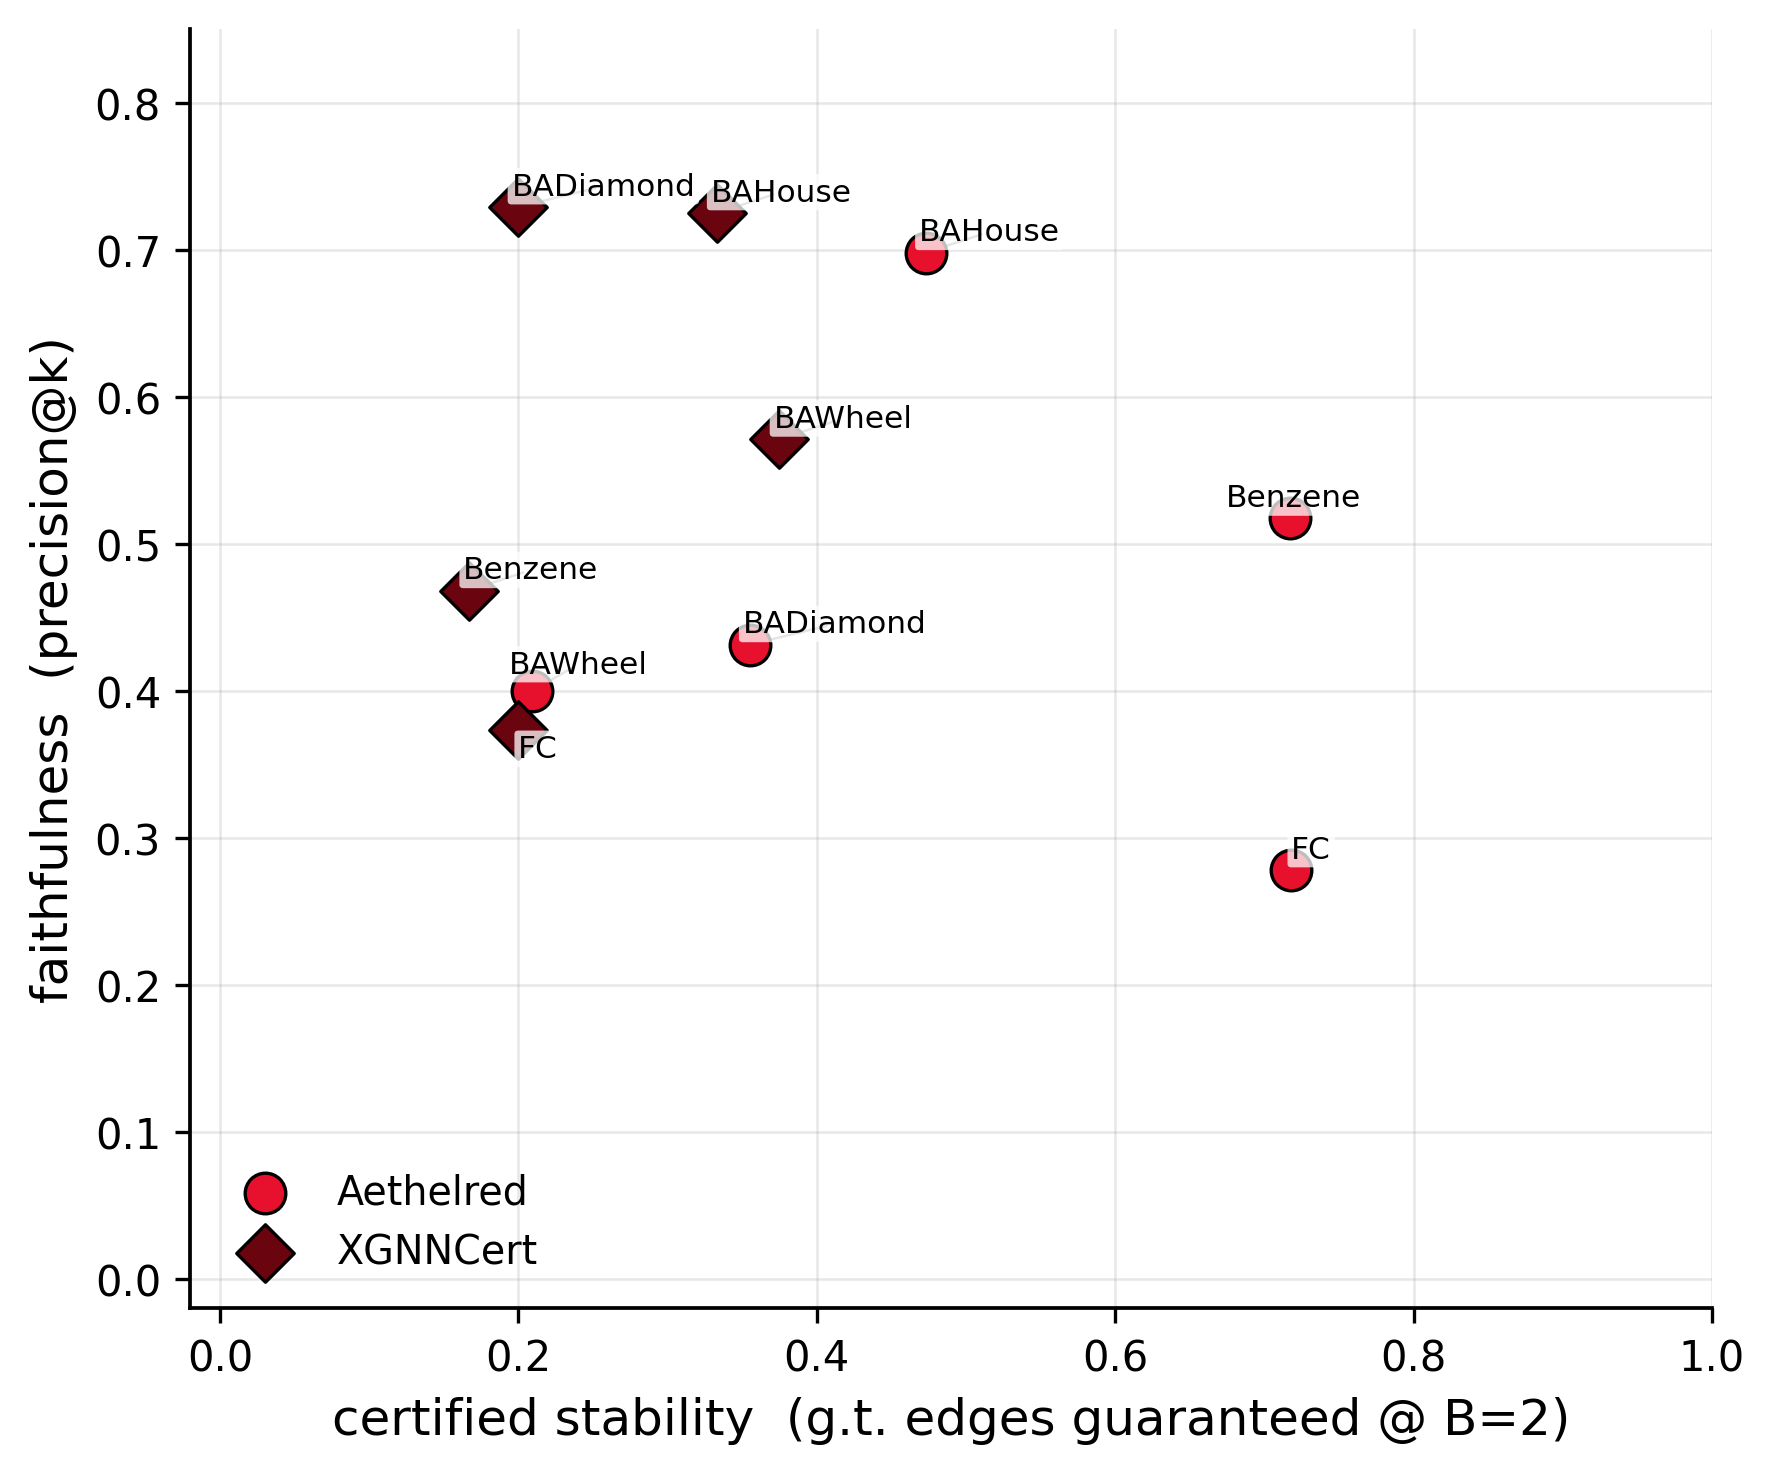
\includegraphics[width=0.85\linewidth]{../../figures/F3_faithfulness_stability_frontier.png}
  \caption{Faithfulness vs.\ certified stability (ground-truth edges guaranteed at
  $B{=}2$). Top-right is best; \xgn{} from published values.}
  \label{fig:frontier}
\end{figure}

\begin{figure}[t]\centering
  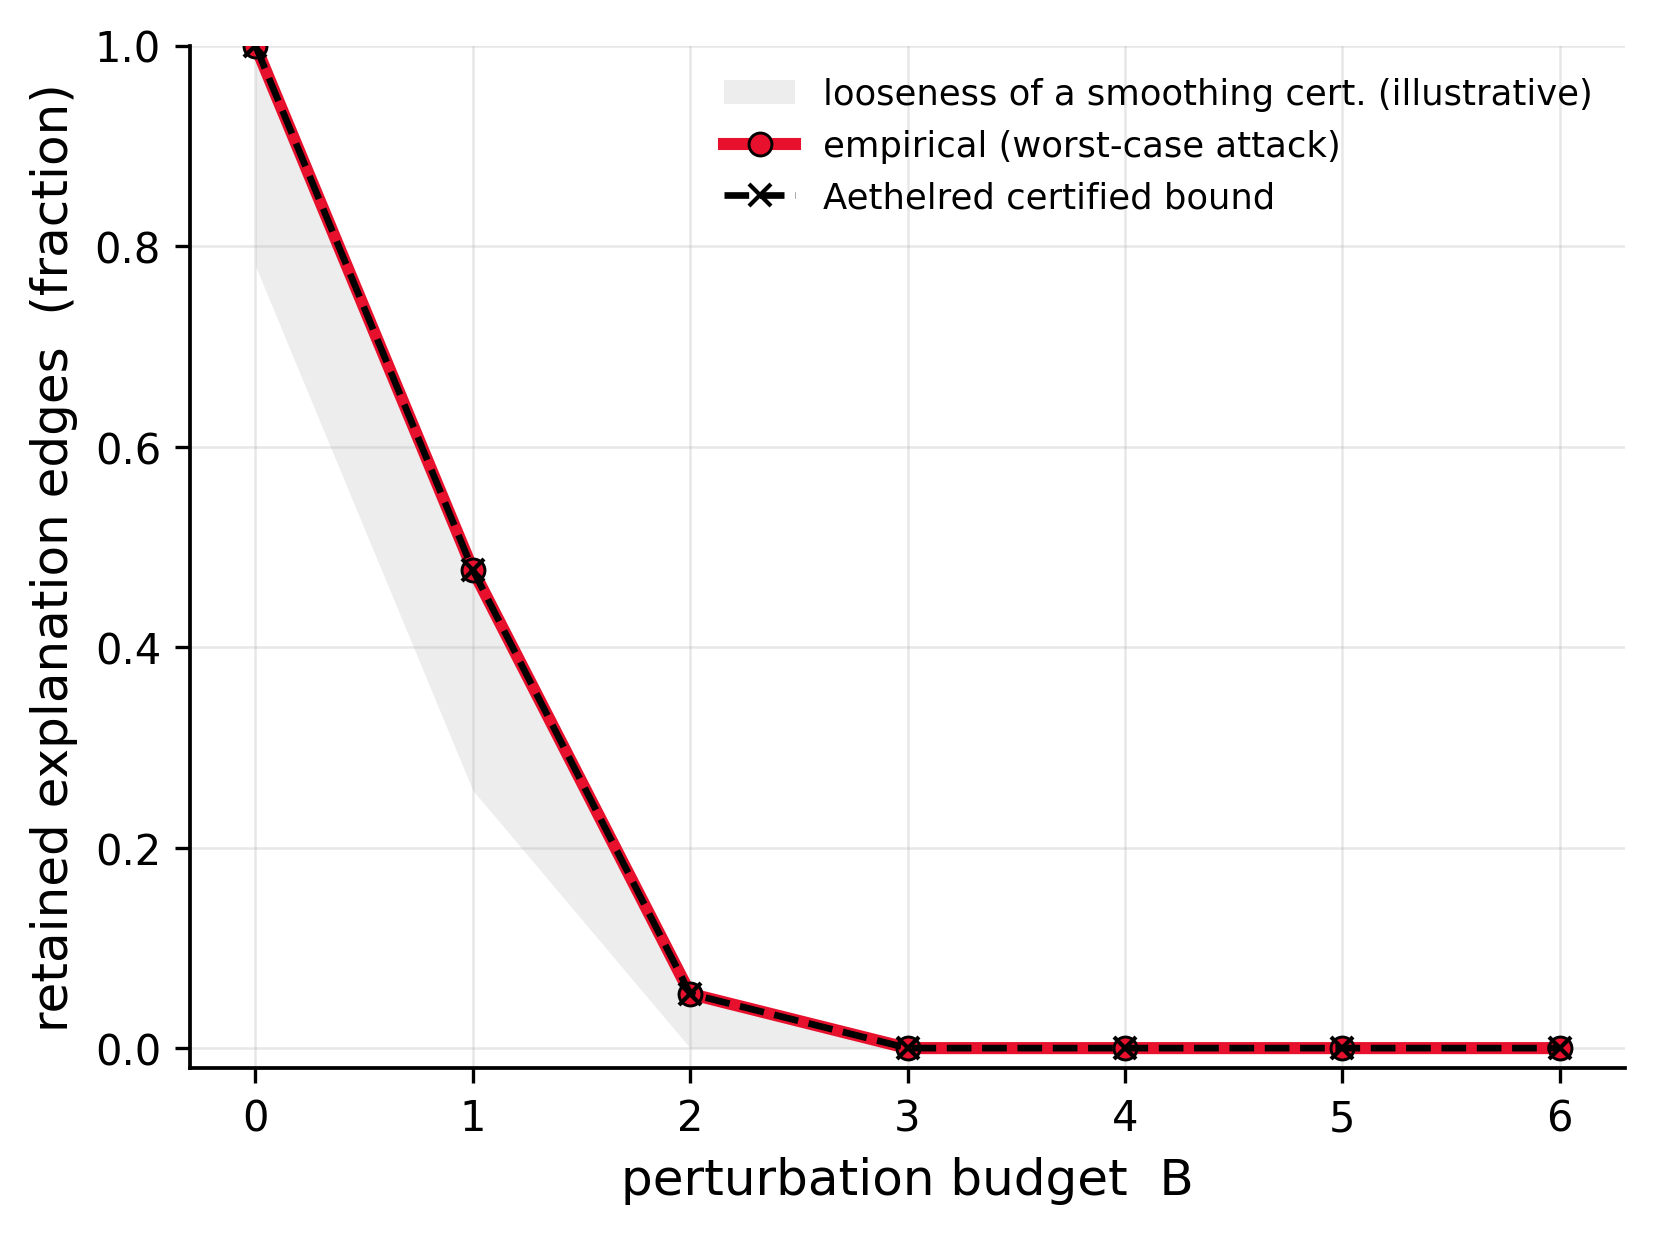
\includegraphics[width=0.82\linewidth]{../../figures/F11_certificate_tightness.png}
  \caption{Tightness: \aeth{}'s certified bound coincides with the empirical
  worst-case (gap $=0$); the grey band marks a smoothing certificate's looseness.}
  \label{fig:tight}
\end{figure}

\begin{figure}[t]\centering
  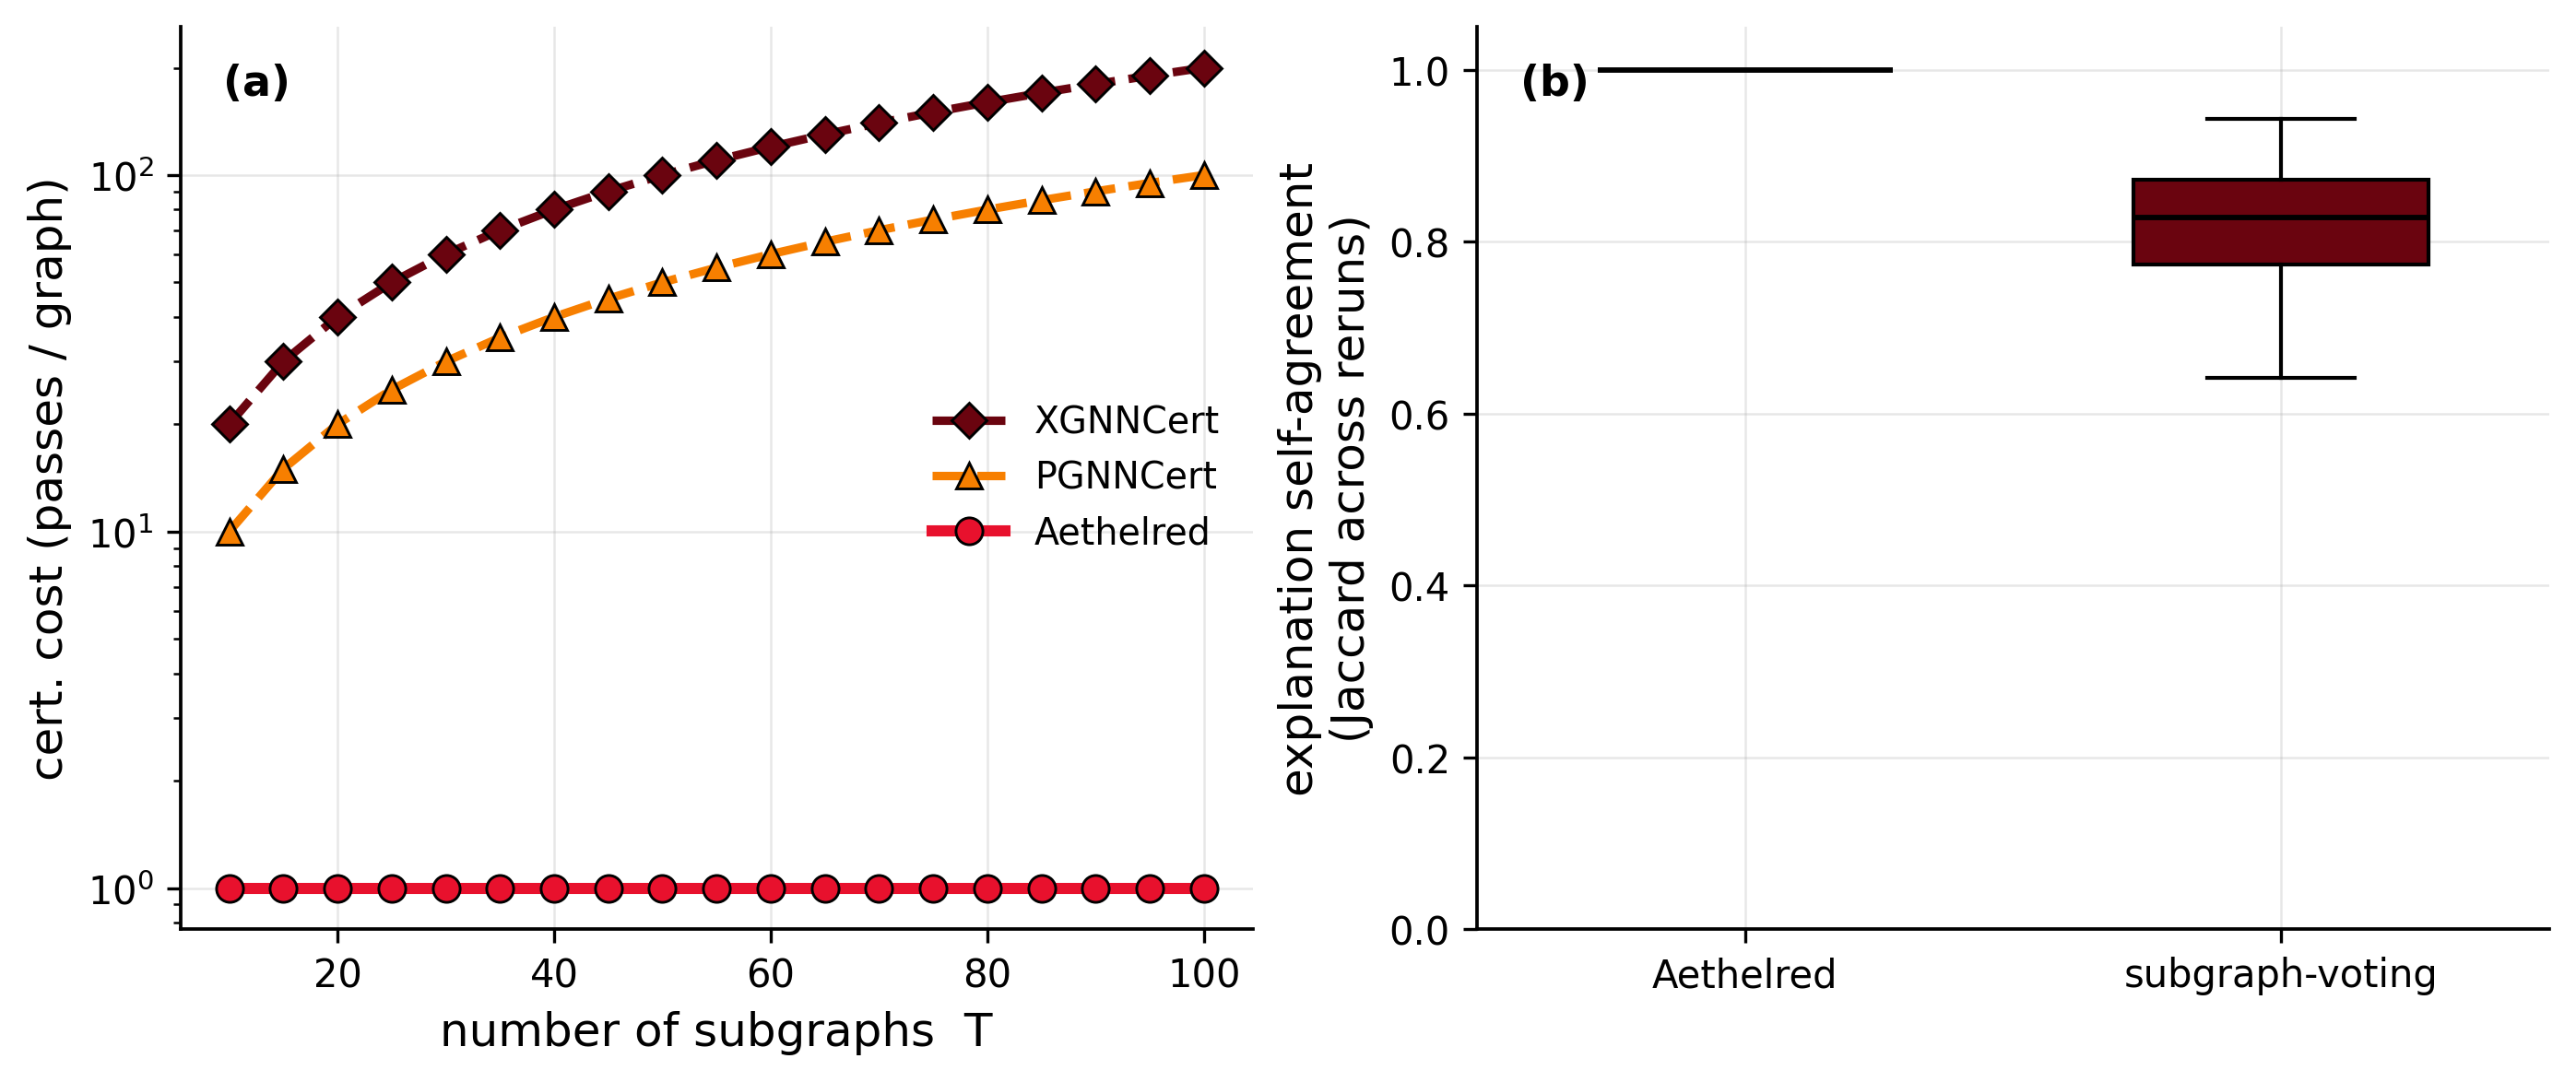
\includegraphics[width=\linewidth]{../../figures/F56_efficiency_determinism.png}
  \caption{(a) Certification cost vs.\ \#sub-graphs $T$ (log scale).
  (b) Explanation self-agreement across reruns.}
  \label{fig:eff}
\end{figure}

\begin{figure}[t]\centering
  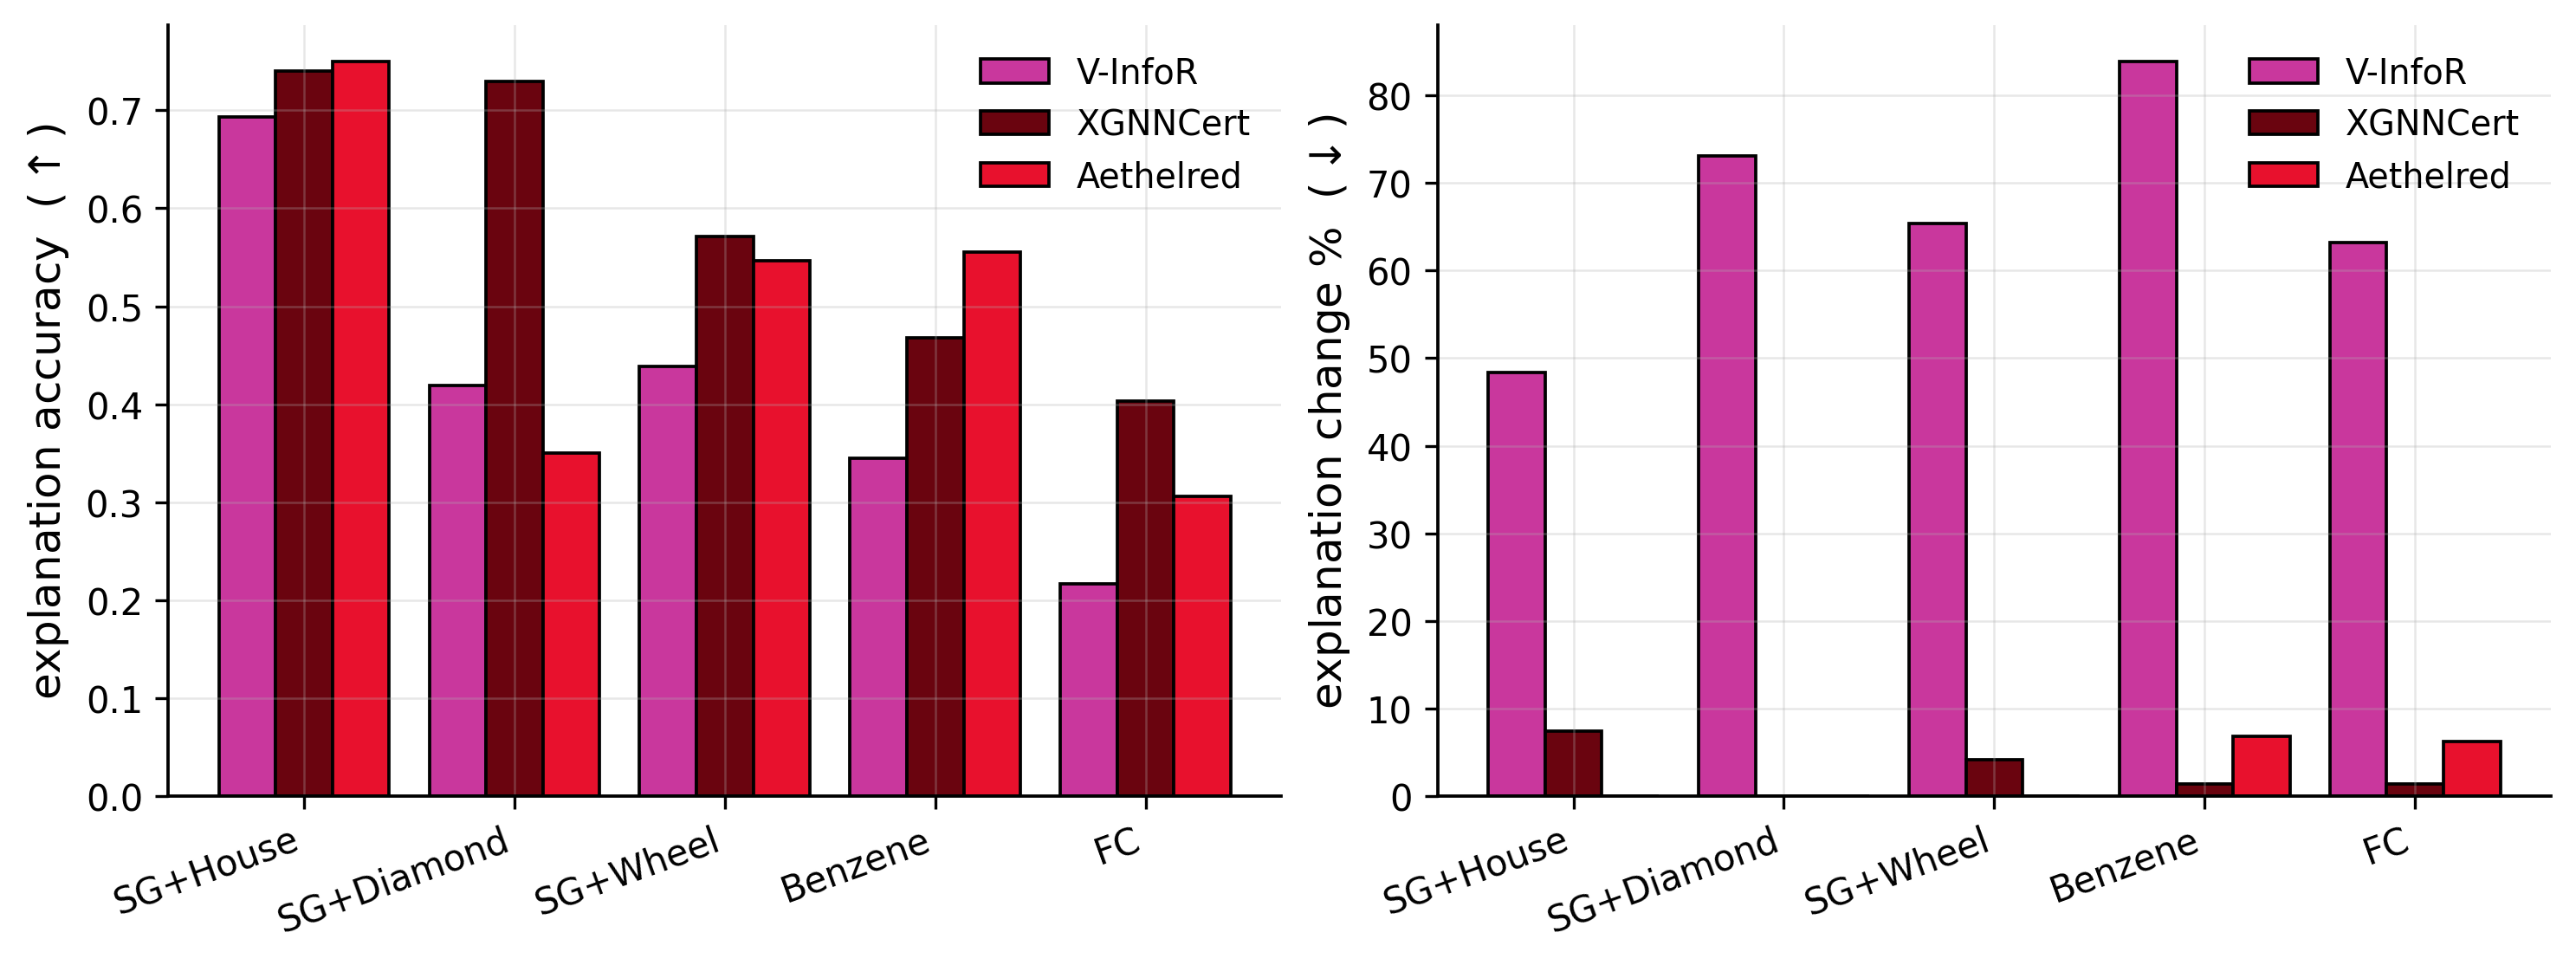
\includegraphics[width=\linewidth]{../../figures/F2b_explanation_robustness_vs_VInfoR.png}
  \caption{Explanation robustness under a $2$-edge attack: faithfulness
  ($\uparrow$) and drift ($\downarrow$) for \aeth{}, \xgn{}, and
  \textcolor{vinfomag}{V-InfoR}.}
  \label{fig:attack}
\end{figure}

\begin{figure}[t]\centering
  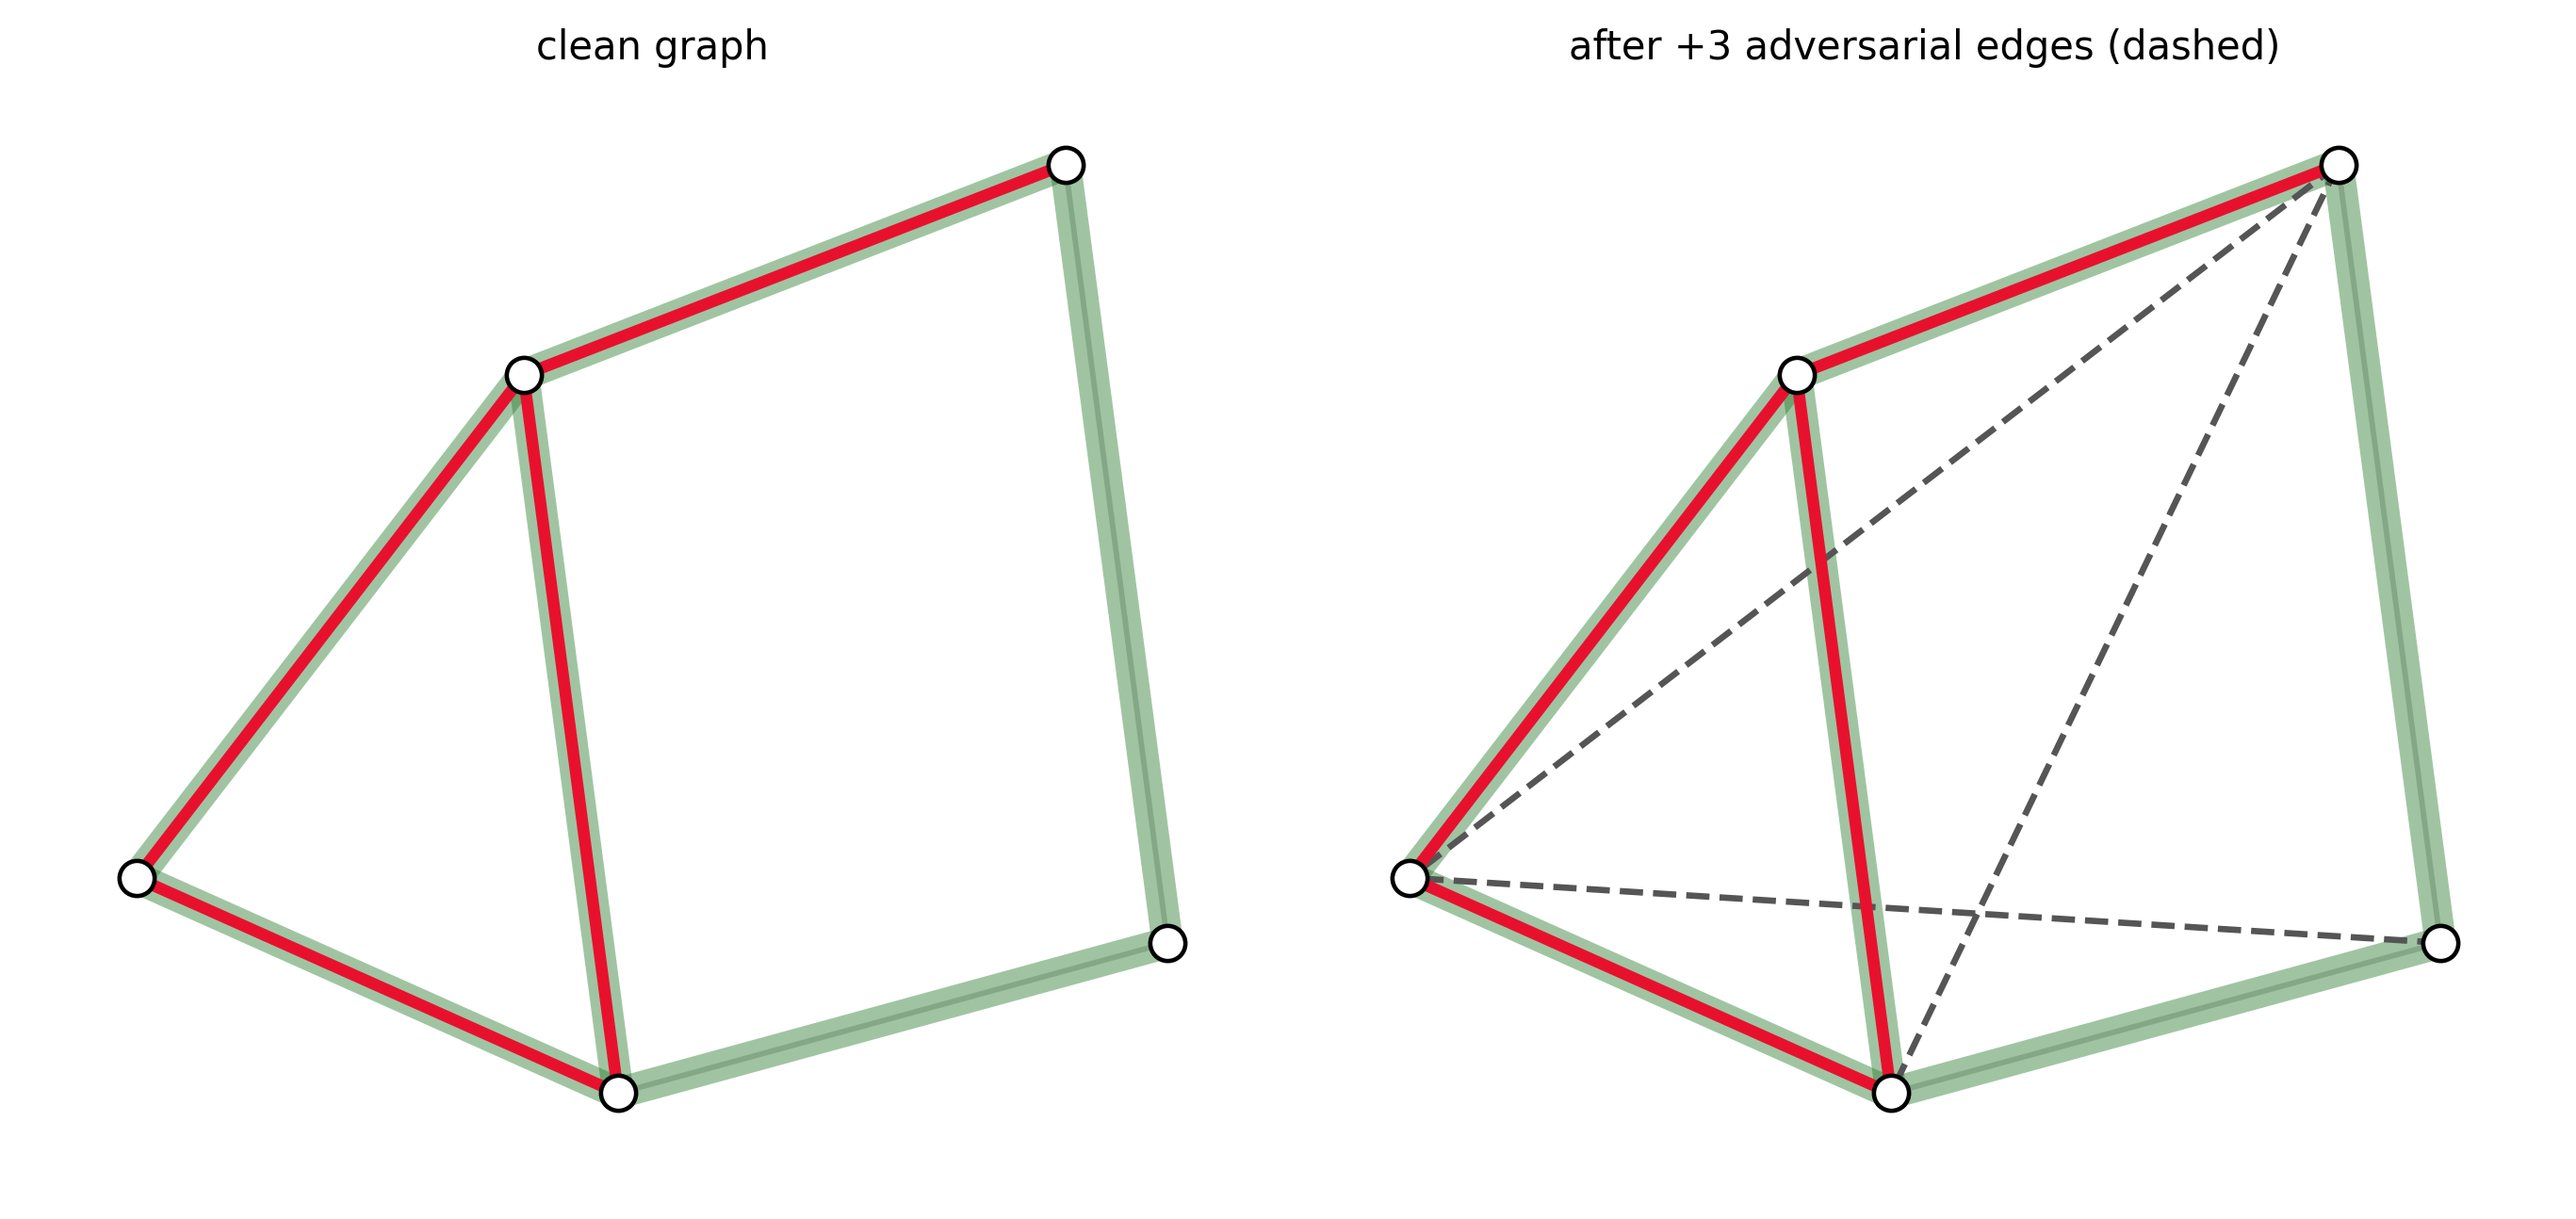
\includegraphics[width=\linewidth]{../../figures/F4_qualitative_explanation.png}
  \caption{\aeth{}'s certified explanation (red) on the ground-truth motif
  (green), before/after $3$ adversarial edges (dashed): the certified subset is
  unchanged.}
  \label{fig:qual}
\end{figure}

\begin{figure}[t]\centering
  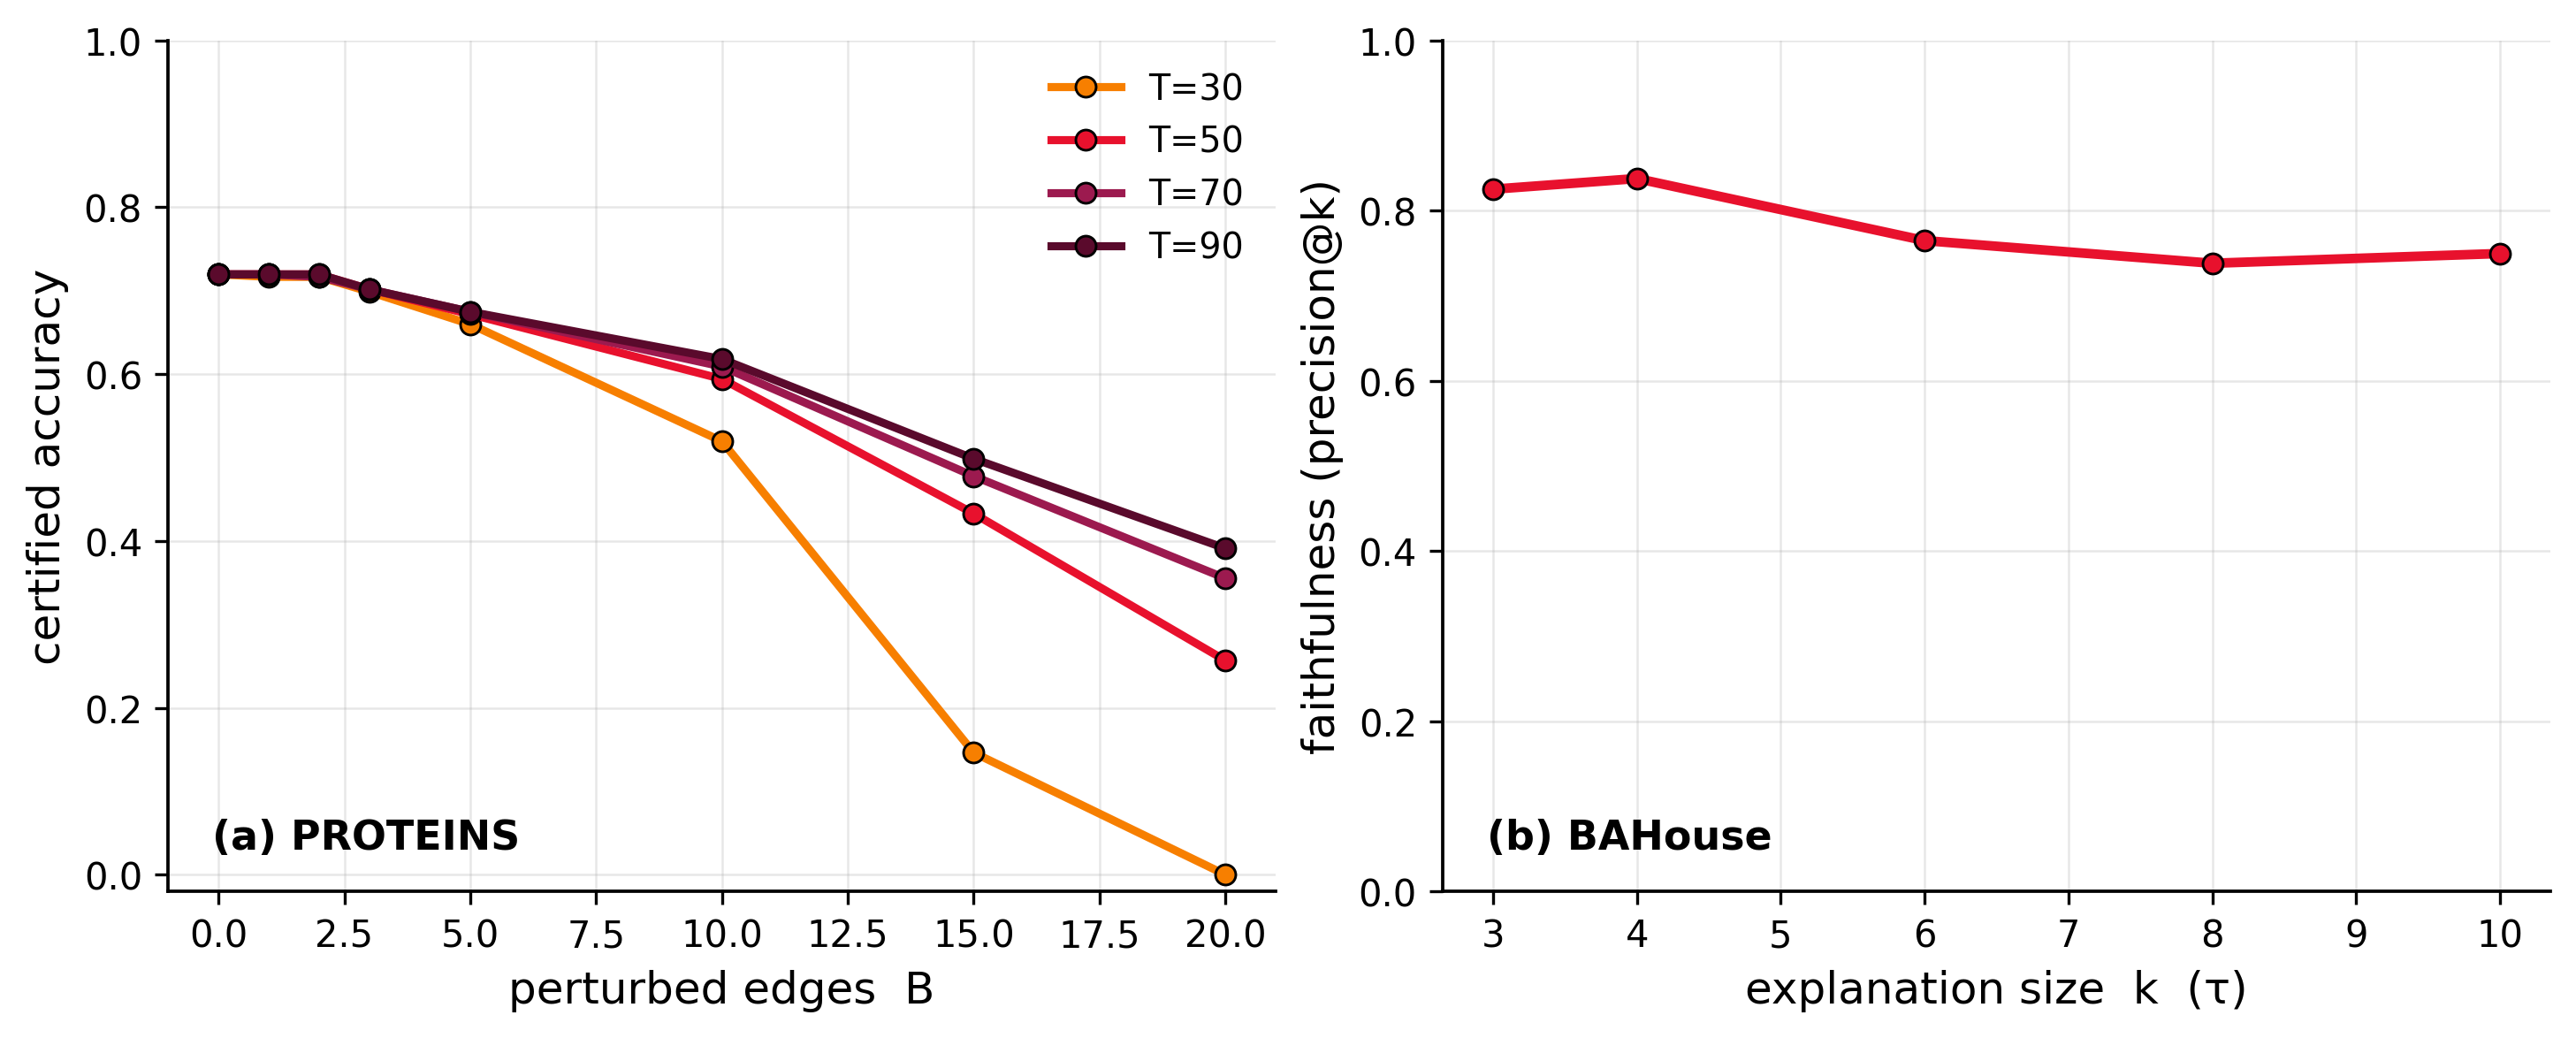
\includegraphics[width=\linewidth]{../../figures/F8_sensitivity.png}
  \caption{(a) Certified accuracy vs.\ budget for $T\!\in\!\{30,50,70,90\}$.
  (b) Faithfulness vs.\ explanation size $k$.}
  \label{fig:sens}
\end{figure}

\begin{figure}[t]\centering
  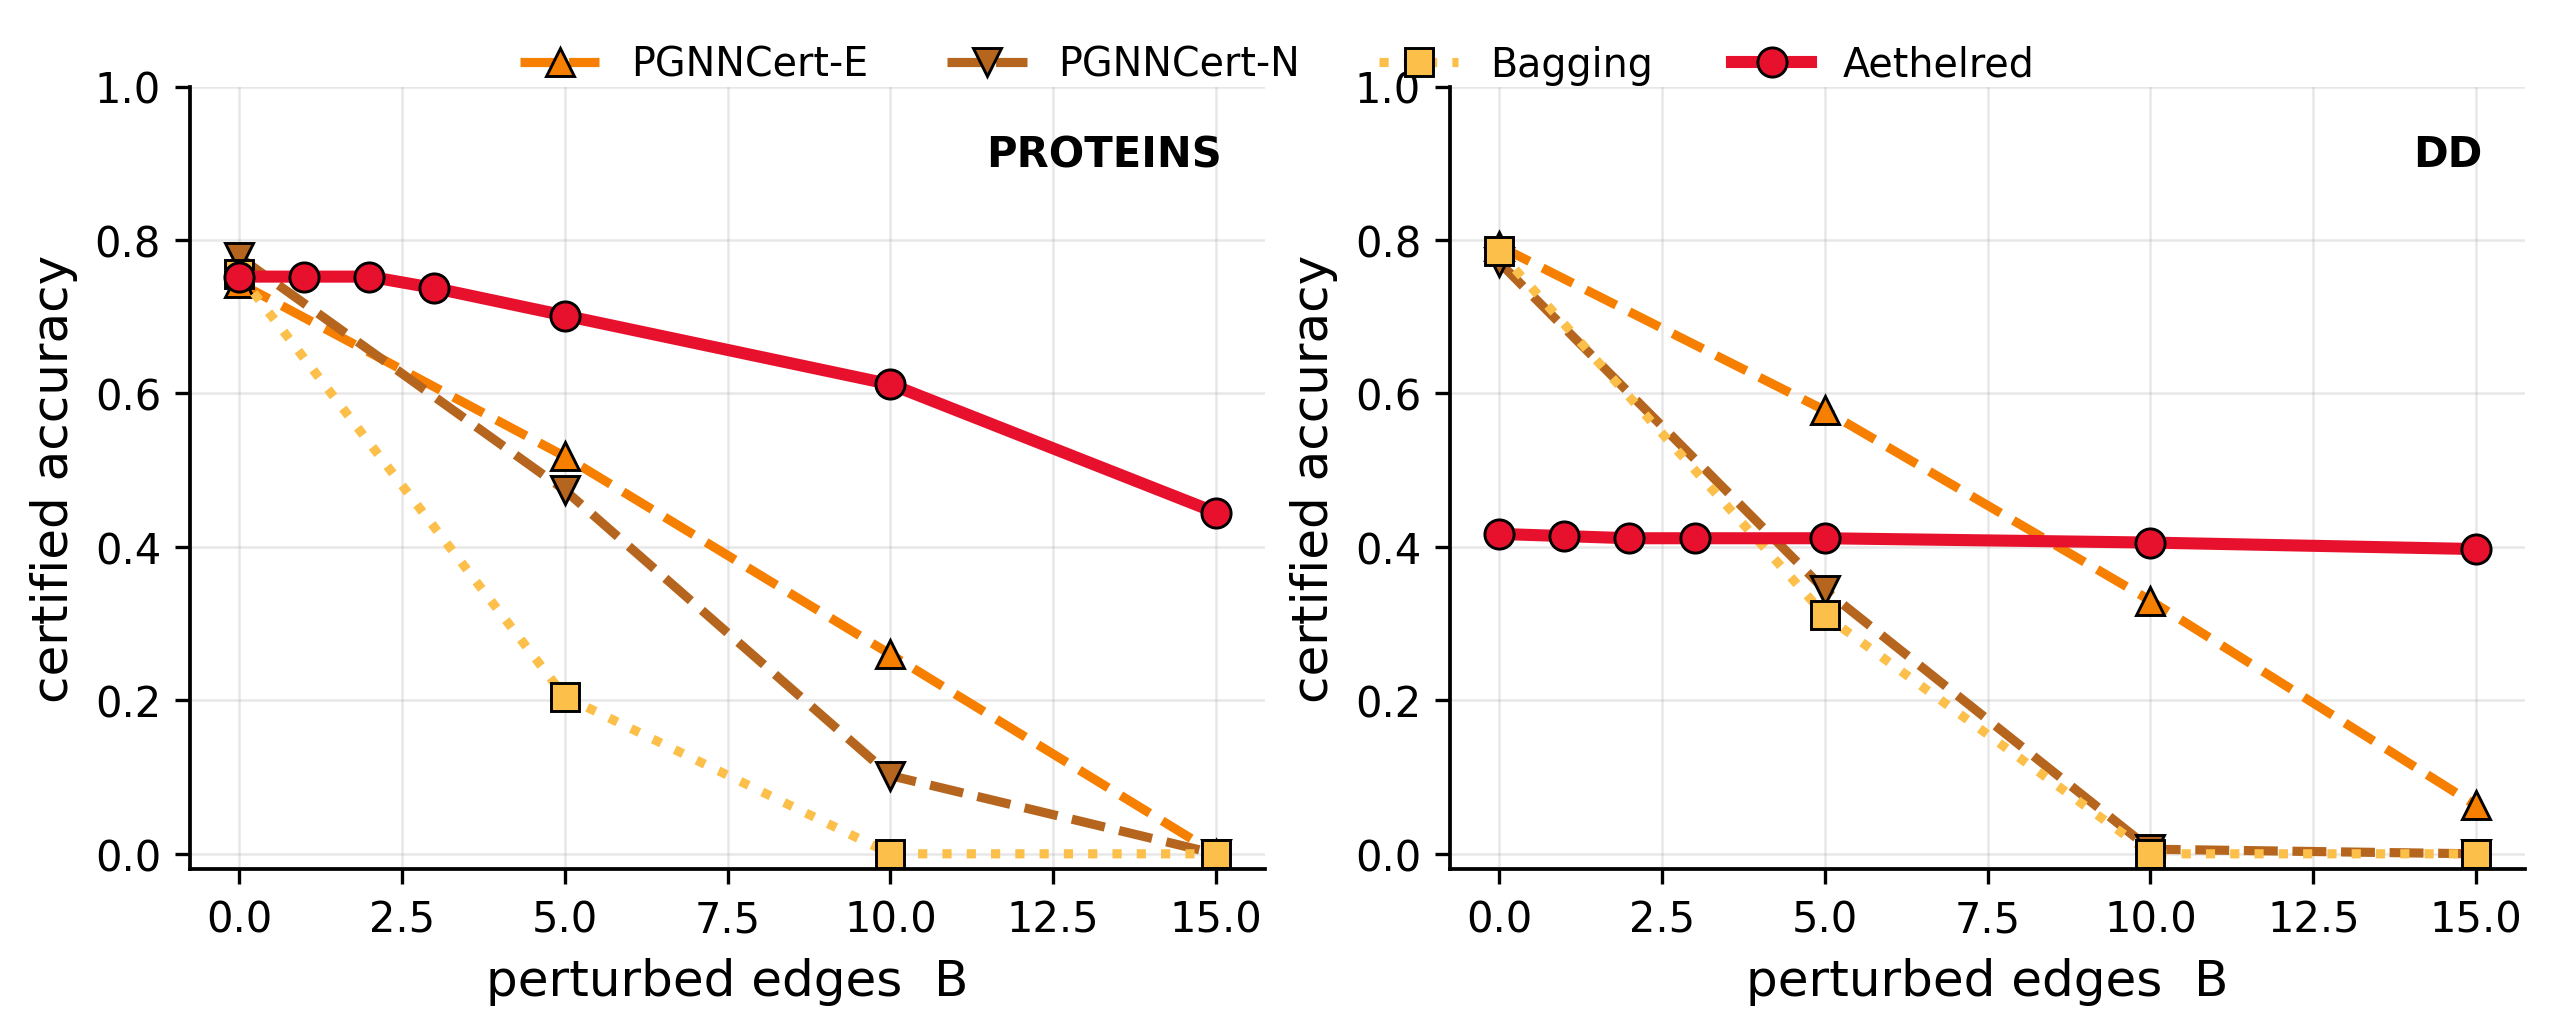
\includegraphics[width=\linewidth]{../../figures/F1_certified_prediction_vs_budget.png}
  \caption{Certified \emph{prediction} accuracy vs.\ edge budget (secondary
  axis), PROTEINS/DD; baselines from \pgn{}'s Table~2.}
  \label{fig:predcert}
\end{figure}

\begin{figure}[t]\centering
  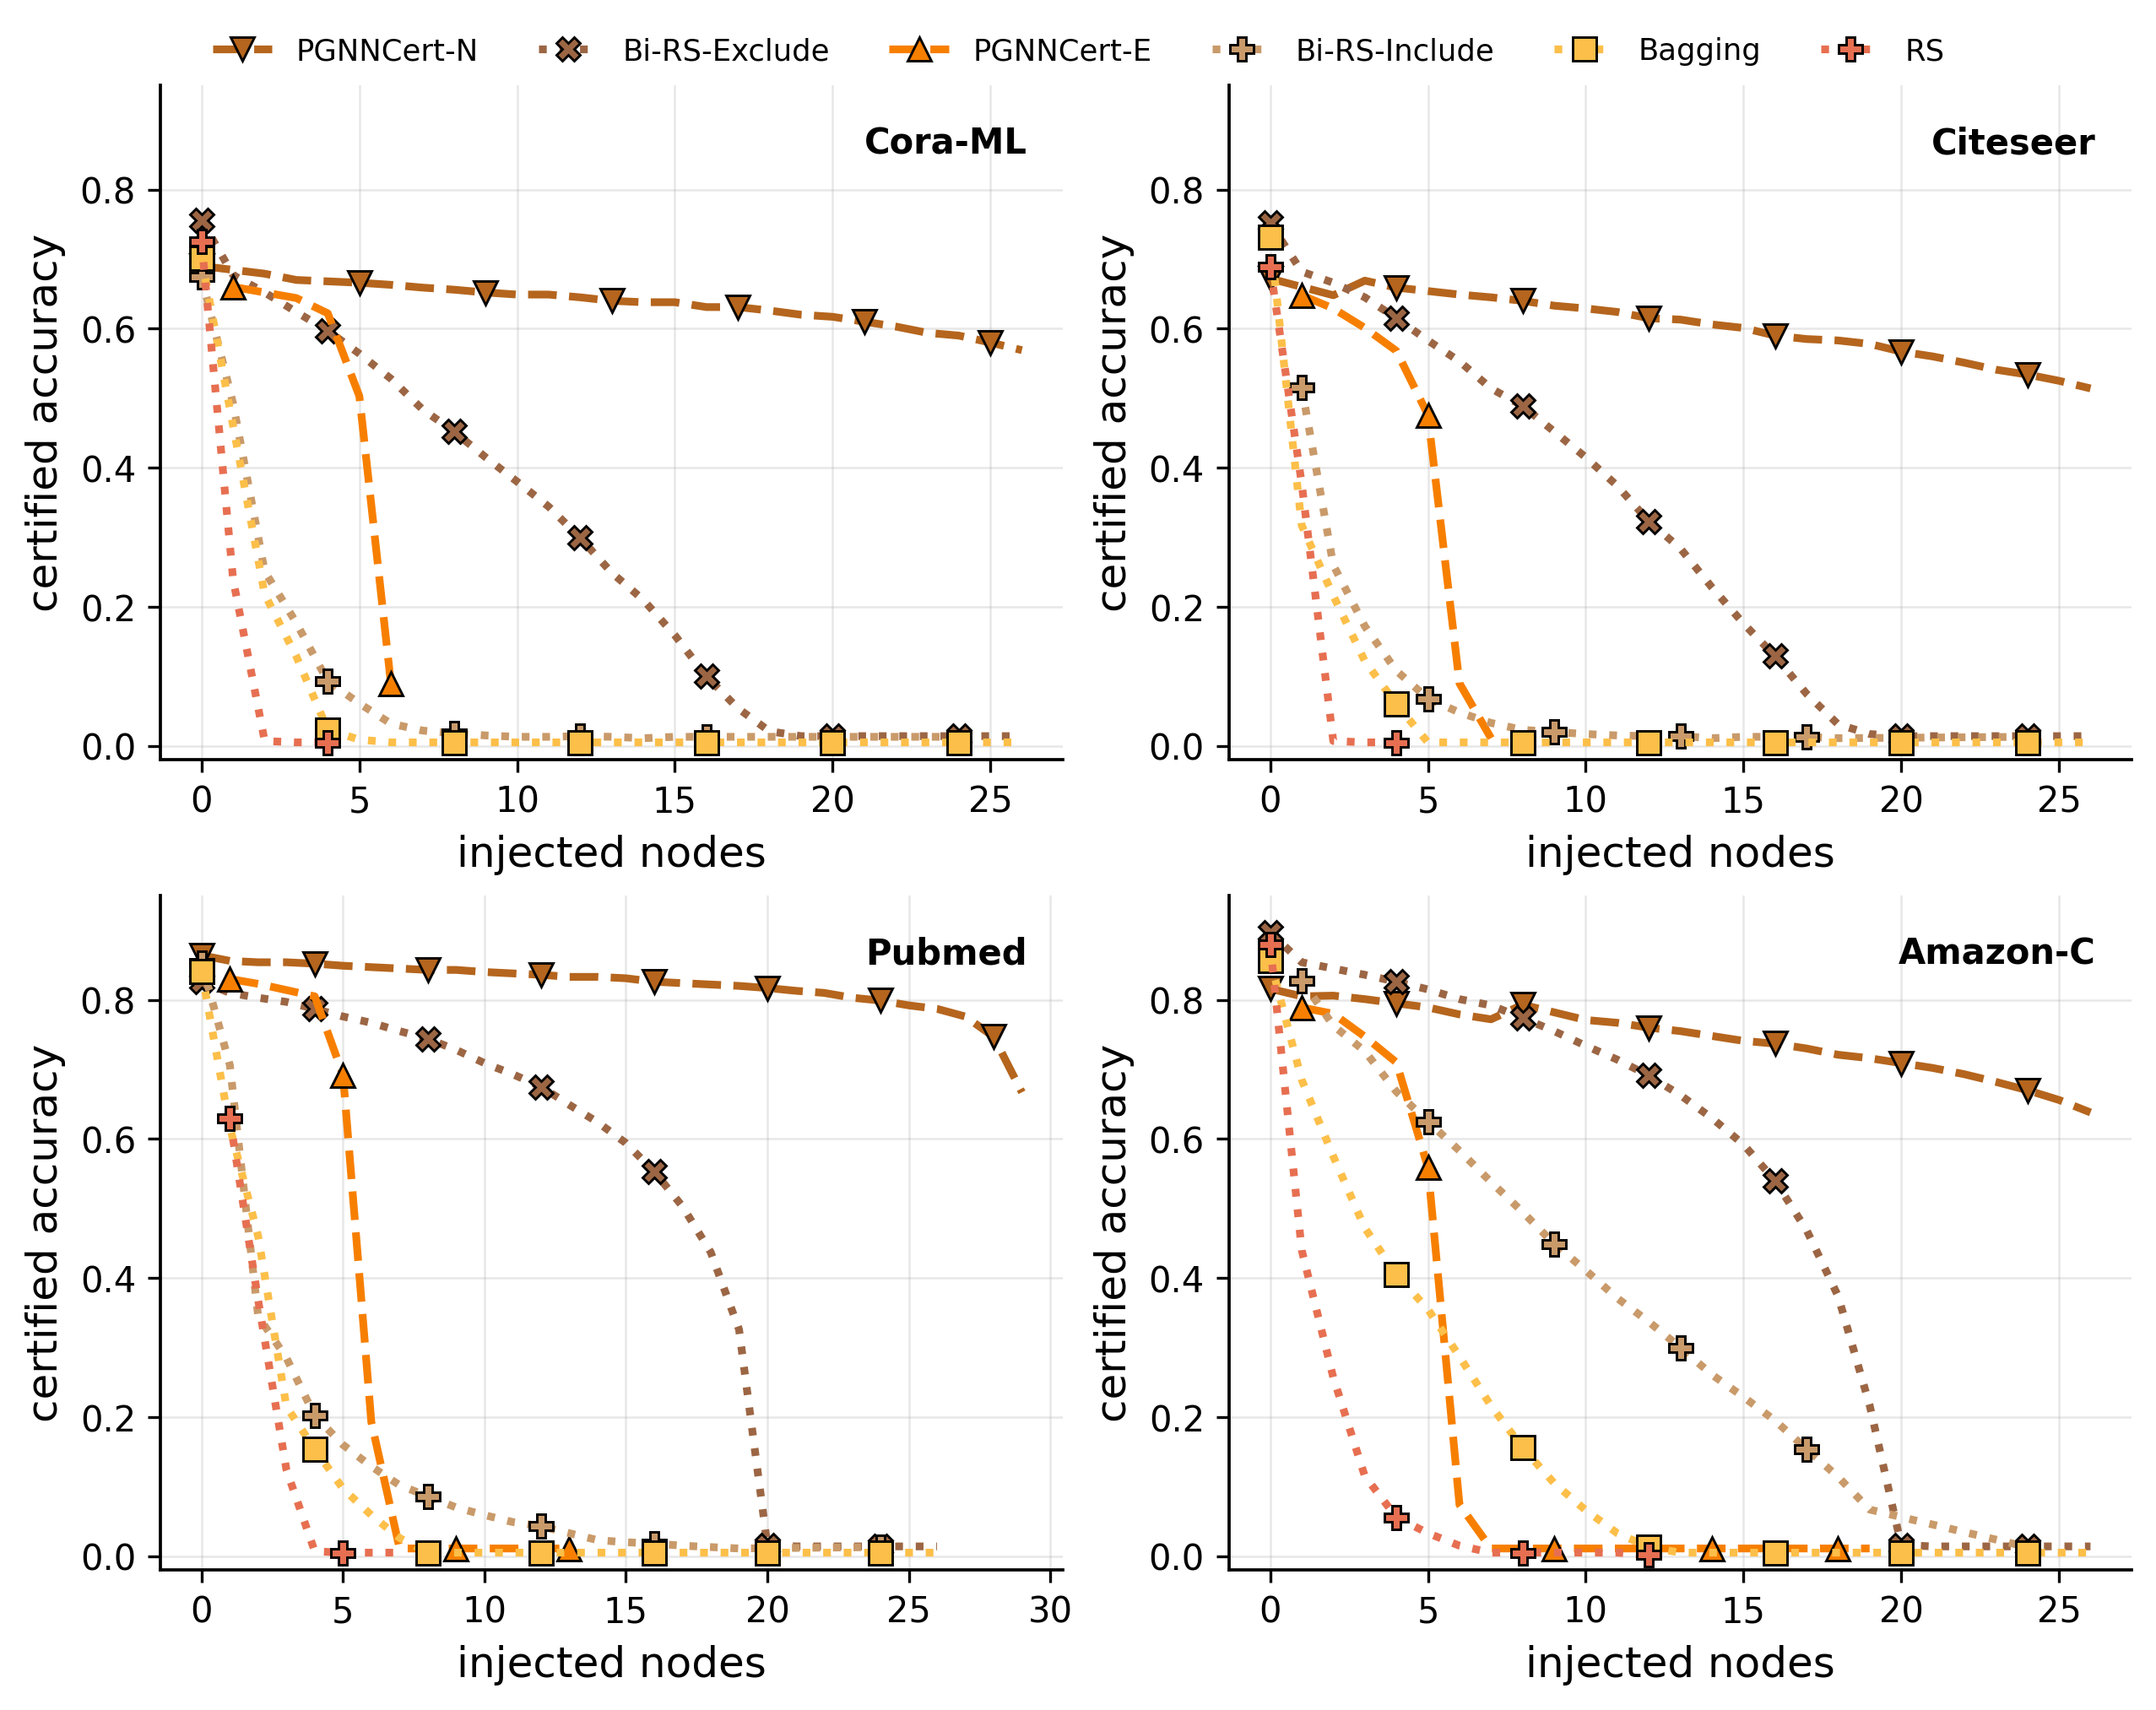
\includegraphics[width=\linewidth]{../../figures/F1b_node_injection_sota.png}
  \caption{Node-injection certified robustness across node datasets---a distinct
  threat model (node classification) shown as field context; \aeth{} targets
  graph-explanation edges.}
  \label{fig:nodeinj}
\end{figure}

\begin{table}[t]\centering
  \caption{Clean accuracy (5 seeds), \aeth{} vs.\ a plain GNN at the baseline's
  learning rate.}
  \label{tab:cleanacc}
  \begin{tabular}{lccc}
    \toprule
    Dataset & Base-GCN & \aeth{}-GCN & $\Delta$ \\
    \midrule
    AIDS & 0.986 & 0.989 & \win{$+0.3$} \\
    MUTAG & 0.762 & 0.769 & \win{$+0.7$} \\
    PROTEINS & 0.740 & 0.764 & \win{$+2.4$} \\
    DD & 0.725 & 0.758 & \win{$+3.4$} \\
    \midrule
    Cora-ML & 0.766 & 0.774 & $+0.8$ \\
    CiteSeer & 0.739 & 0.721 & \cav{$-1.7$} \\
    PubMed & 0.867 & 0.863 & $-0.4$ \\
    Amazon-C & 0.883 & 0.879 & $-0.3$ \\
    \bottomrule
  \end{tabular}
\end{table}
